\documentclass{article}

% Recommended, but optional, packages for figures and better typesetting:
\usepackage{microtype}
\usepackage{graphicx}
\usepackage{tabularx}
\usepackage{subfigure}
\usepackage{booktabs} % for professional tables
\usepackage{makecell}
\usepackage{caption}
\usepackage{hyperref}


% Attempt to make hyperref and algorithmic work together better:
\newcommand{\theHalgorithm}{\arabic{algorithm}}

% For theorems and such
\usepackage{amsmath} \usepackage{amssymb} \usepackage{mathtools} \usepackage{amsthm}

% if you use cleveref..
\usepackage[capitalize,noabbrev]{cleveref}

%%%%%%%%%%%%%%%%%%%%%%%%%%%%%%%%
% THEOREMS
%%%%%%%%%%%%%%%%%%%%%%%%%%%%%%%%
\theoremstyle{plain}
\newtheorem{theorem}{Theorem}[section]
\newtheorem{proposition}[theorem]{Proposition}
\newtheorem{lemma}[theorem]{Lemma}
\newtheorem{question}[theorem]{Question}
\newtheorem{corollary}[theorem]{Corollary}
\newtheorem{fact}[theorem]{Fact}
\theoremstyle{definition}
\newtheorem{definition}[theorem]{Definition}
\newtheorem{assumption}[theorem]{Assumption}
\theoremstyle{remark}
\newtheorem{remark}[theorem]{Remark}

% Todonotes is useful during development; simply uncomment the next line
%    and comment out the line below the next line to turn off comments
%\usepackage[disable,textsize=tiny]{todonotes}
\usepackage[textsize=tiny]{todonotes}




\DeclareMathOperator{\polylog}{polylog}
\DeclareMathOperator{\cost}{cost}
\DeclareMathOperator{\dist}{dist}
\DeclareMathOperator{\poly}{poly}


\newcommand{\R}{\mathbb{R}}
\newcommand{\E}{\mathbb{E}}
\newcommand{\coreset}{\Omega}
\newcommand{\calC}{\mathcal C}
\newcommand{\calD}{\mathcal D}
\newcommand{\calS}{\mathcal S}
\newcommand{\calA}{\mathcal A}
\newcommand{\opt}{\text{OPT}}
\newcommand{\eps}{\varepsilon}

\newcommand{\fkmeans}{\textsc{Fast-kmeans++}~}

\newcommand{\lpar}{\left(}
\newcommand{\rpar}{\right)}
\newcommand{\lbra}{\left\{}
\newcommand{\rbra}{\right\}}
\newcommand{\lnor}{\left\|}
\newcommand{\rnor}{\right\|}


\newcounter{sideremark}
\newcommand{\marrow}{\stepcounter{sideremark}\marginpar{$\boldsymbol{
\longleftarrow\scriptstyle\arabic{sideremark}}$}}

 \newcommand{\david}[1]{
 %  \ifdraft{
    \textsf{{\color{blue} *** (David) \marrow #1 ***}}
 %  }
 %  \fi
 }
  \newcommand{\andrew}[1]{
 %  \ifdraft{
    \textsf{{\color{red} *** (Andrew) \marrow #1 ***}}
 %  }
 %  \fi
 }
 
   \newcommand{\chris}[1]{
 %  \ifdraft{
    \textsf{{\color{green} *** (Chris) \marrow #1 ***}}
 %  }
 %  \fi
 }

 
%for having enumerates with (i) (ii) (iii): 
\renewcommand{\labelenumi}{\theenumi}
 
% if you need to pass options to natbib, use, e.g.:
%     \PassOptionsToPackage{numbers, compress}{natbib}
% before loading neurips_2023


% ready for submission
%\usepackage{neurips_2023}


% to compile a preprint version, e.g., for submission to arXiv, add add the
% [preprint] option:
%     \usepackage[preprint]{neurips_2023}


% to compile a camera-ready version, add the [final] option, e.g.:
%     \usepackage[final]{neurips_2023}


% to avoid loading the natbib package, add option nonatbib:
\usepackage{neurips_2023}


\usepackage[utf8]{inputenc} % allow utf-8 input
\usepackage[T1]{fontenc}    % use 8-bit T1 fonts
\usepackage{hyperref}       % hyperlinks
\usepackage{url}            % simple URL typesetting
\usepackage{booktabs}       % professional-quality tables
\usepackage{amsfonts}       % blackboard math symbols
\usepackage{nicefrac}       % compact symbols for 1/2, etc.
\usepackage{microtype}      % microtypography
\usepackage{xcolor}         % colors
\usepackage{algorithm}
\usepackage[noend]{algpseudocode}


\title{Settling Time vs. Accuracy Tradeoffs for Clustering Big Data}


% The \author macro works with any number of authors. There are two commands
% used to separate the names and addresses of multiple authors: \And and \AND.
%
% Using \And between authors leaves it to LaTeX to determine where to break the
% lines. Using \AND forces a line break at that point. So, if LaTeX puts 3 of 4
% authors names on the first line, and the last on the second line, try using
% \AND instead of \And before the third author name.


\author{%
  David S.~Hippocampus\thanks{Use footnote for providing further information
    about author (webpage, alternative address)---\emph{not} for acknowledging
    funding agencies.} \\
  Department of Computer Science\\
  Cranberry-Lemon University\\
  Pittsburgh, PA 15213 \\
  \texttt{hippo@cs.cranberry-lemon.edu} \\
  % examples of more authors
  % \And
  % Coauthor \\
  % Affiliation \\
  % Address \\
  % \texttt{email} \\
  % \AND
  % Coauthor \\
  % Affiliation \\
  % Address \\
  % \texttt{email} \\
  % \And
  % Coauthor \\
  % Affiliation \\
  % Address \\
  % \texttt{email} \\
  % \And
  % Coauthor \\
  % Affiliation \\
  % Address \\
  % \texttt{email} \\
}


\begin{document}


\maketitle


\begin{abstract}
We study the theoretical and practical limits of $k$-means and $k$-median clustering on large datasets. Since the reader's favorite clustering method is likely
slower than $\tilde{O}(nd)$ time, the general approach is to compress the data and perform the clustering on the compressed representation. Towards this goal,
the number of features can be reduced in effectively linear time with guaranteed accuracy using random projections. Unfortunately, there is no such universal
best choice for compressing the number of points -- while random sampling runs in sublinear time and coresets provide theoretical guarantees, the former does
not enforce accuracy while the latter is too slow as $n$ and $k$ grow. Indeed, it has been conjectured that any sensitivity-based coreset construction
necessitates $\tilde{O}(nd + nk)$ time.

We examine this relationship by first showing that there does exist an algorithm that obtains coresets via sensitivity sampling in $\tilde{O}(nd)$ time --
within log-factors of the time it takes to read the data.  Any approach that significantly improves on this must then resort to practical heuristics, leading us
to consider the spectrum of sampling strategies across both real and artificial datasets in the static and streaming settings. Through this, we show the
conditions in which coresets are necessary for preserving cluster validity as well as the settings in which faster, cruder sampling strategies are sufficient.
As a result, we provide a comprehensive theoretical and practical blueprint for clustering effectively regardless of data size.  Our (anonymized) code is
publicly available at \textcolor{blue}{\href{https://anonymous.4open.science/r/Fast-Coreset-Generation-7564}{source}}.
\end{abstract}


\section{Introduction}

The modern data analyst has no shortage of clustering algorithms to choose from but, given the ever-increasing size of relevant datasets, many are often
too slow to be practically useful. This has prompted the rise of big data algorithms which provide both theoretical guarantees and
practical improvements for standard data-science techniques on otherwise insurmountable datasets. The perspectives
of theoretical soundness and practical efficacy are, however, slightly at odds with one another. On the one hand, theoretical guarantees provide assurance that
the algorithm will obtain valid solutions without unlucky inputs affecting their runtime or accuracy. On the other hand, it is sometimes difficult to convince
oneself to implement the theoretically optimal algorithm when there are cruder methods that are faster to get running and perform well in practice.

Since datasets can be large in the number of points $n$ and/or the number of features $d$, big-data methods must mitigate the effects of both.
With respect to the feature space, the question is effectively closed as random projections are fast (running in effectively linear time), practical to
implement, and provide tight guarantees on the embedding's size and quality. The outlook is less clear when reducing the number of points $n$, and there are
two separate paradigms that each provide distinct advantages.  On the one hand we have uniform sampling, which runs in sublinear time but may miss important subsets of
the data and therefore cannot guarantee accuracy.  On the other hand the most accurate sampling strategies are those that provide the \emph{strong coreset}
guarantee, wherein the cost of any solution on the compressed data is within an $\varepsilon$-factor of that solution's cost on the original dataset.
Surprisingly, many coreset constructions can remove the dependency on $n$, significantly accelerating downstream tasks.

We study both paradigms with respect to a classic problem -- what are the limits and possibilities of compression for the $k$-means and $k$-median objectives?
Whereas uniform sampling provides optimal speed but no accuracy guarantee, coreset constructions have
unclear runtime bounds despite their tight bounds on the minimum number of samples required for accurate compression. Although there is little to study with respect to random
sampling, the lack of clarity regarding linear-time coreset constructions throws into question their ability to facilitate clustering on large datasets. Indeed,
available linear-time coreset via sensitivity sampling obtain an additive error \cite{BachemL018} while other fast sampling strategies
\cite{kmeans_sublinear_bachem16} have weaker guarantees. Recently, \cite{DSWY22} proposed a sensitivity-based method for strong coresets that runs in time
$\tilde{O}(nd + nk)$ and conjectured this to be optimal for $k$-median and $k$-means.  Since the issue of determining an optimal coreset size has recently
been resolved \cite{CSS21,CLSSS22,HLW23}, this is arguably the main open problem in coreset research for center-based clustering. We resolve this by showing that
there exists an easy-to-implement algorithm that constructs coresets in $\tilde{O}(nd)$ time -- only logarithmic factors away from the time it takes to read in
the dataset.

Nonetheless, this does not fully illuminate the landscape between the sampling paradigms for clustering algorithms when applying them in practice. Although our algorithm achieves an optimal
running time, it is certainly possible that other, cruder methods may be just as viable on most real world data sets despite having no worst case guarantees.
Thus, there is a natural spectrum within linear-time algorithms where obtaining more information about the dataset allows for a better
sampling strategy at the expense of sublinear factors in speed. We state this formally in the following question: When are optimal $k$-means and $k$-median
coresets necessary and what is the practical tradeoff between coreset speed and accuracy? To this end, we show that while many practical settings do not require
the full coreset guarantee, one cannot cut corners if one wants to be confident in their compression. We also
show that this extends to the streaming data paradigm and applies to downstream clustering approaches.

\section{Preliminaries and Related Work}
\label{sec:preliminaries}

\paragraph*{On Sampling Strategies.}
\label{ssec:sens_sampling}

As discussed, we focus our study on linear- and sublinear-time sampling strategies. Specifically, given a dataset $P \in \R^{n \times d}$, we want to sample
$\Omega \in \R^{m \times d} \subset P$ such that $m \ll n$ along with a weights vector $w \in \R^m$. The goal is then that for some solution $\calC$, $\Omega$
provides us with an idea of the solution's quality with respect to the original dataset, i.e. $\sum_{p \in \Omega} w_p \cost(p, \calC) \sim \sum_{p \in P}
\cost(p, \calC)$.  The quickest sampling strategy, running in sublinear time, is uniform sampling. It is clear, however, that this cannot provide any
cost-preservation guarantee as missing a single extreme outlier will cause the sampling strategy to fail. Thus, any approach that outperforms this strategy must
read in the entire dataset and therefore run in at least linear time. Indeed, sublinear algorithms always require some assumption on the input to provide
guarantees, see \cite{Ben-David07,czumaj2007sublinear,HJJ23,meyerson2004k}.


Among these more sophisticated sampling strategies, coresets offer the strongest compression guarantee. Specifically, a strong $\eps$-coreset is an 
$\Omega
\subseteq P$ with weights $\tilde w$ such that for \emph{any} solution $\calC$, \[\sum_{p \in \Omega} \tilde w_p \cost(p, \calC) \in (1 \pm \eps) \cost(P, \calC)\] with
high probability.  Going forward, we will discuss this in the context of the $k$-median and $k$-means cost functions: for dataset $P \in \R^d$ with weights $w
: P \rightarrow \R^+$, and any $k$-tuple $\calC$ in $\R^d$, \[\cost_z(P, \calC) := \sum_{p \in P} \tilde w(p) \dist^z(p, \calC),\] with
$z=1$ for $k$-median and $z=2$ for $k$-means. We use $\opt$ to denote $\min_{\Omega} \cost_z(P, \calC)$.

Recently, sampling with respect to sensitivity values has grown to prominence due to its simplicity and coreset guarantee.  True sensitivity values are defined
as $\sup_{\calC} \frac{\dist^z(p, \calC)}{\cost_z(P, \calC)}$, where the supremum is taken over all possible solutions $\calC$. Intuitively, this is a measure
of the maximum impact a point can have on a solution and is difficult to evaluate directly.
Thus, the approximate sensitivity-sampling algorithm we consider is the following, as introduced in \cite{FeldmanL11}.
Given an $\alpha$-approximate solution to a clustering problem $\calC$, importance scores are defined as
\begin{equation}
\label{eq:sensitivity}
\sigma_\calC(p) = \alpha \cdot \left( \dfrac{\cost(p, \calC)}{\cost(\calC_{p}, \calC)} + \dfrac{1}{|\calC_p|} \right),
\end{equation}
where $\calC_p$ is the cluster that $p$ belongs to. This is always an upper-bound on the sensitivity values, see \cite{FL11,FeldmanSS20}.

The coreset $\Omega$ then consists of $m$ points sampled proportionate to $\sigma$ with weights defined as follows. First, for any sampled point $p$, define $w_p :=
\frac{1}{\Pr[p \in \Omega]} = \frac{\sum_{p'} s_\calC(p')}{m s_\calC(p)}$. For a cluster $C_i$, let $|\hat{C_i}|$ be the number of points in $C_i$ estimated by the
sample, i.e. $C_i \cap \Omega$ weighted with $w_p$. A sampled point $p$ in $C_i$ is
weighted $\tilde w(p) = \tilde w_1(p) \lpar (1+\eps)|C_i| - |\hat{C_i}|\rpar$.  \cite{FeldmanL11} and subsequent works showed that, when $\calC$ is
a $O(1)$-approximation, sampling $\Omega = \tilde O\lpar k \eps^{-2z-2}\rpar$ many points was enough to ensure concentration, namely, $\Omega$ is a coreset with
probability at least $2/3$.

To perform this algorithm, the bottleneck in the running time lies in computing the solution $\calC$ as well as then obtaining costs of every point to its
assigned center in $\calC$. Using any bicriteria approximation algorithm\footnote{For $k$-means an $(\alpha,\beta)$ bicriteria approximation is an algorithm
that computes a solution $\calC$ satisfying $\cost(P\calC)\leq \alpha\cdot \opt$ and $|\calC|\leq \beta\cdot k$.} such as the standard $k$-means++ algorithm
\cite{ArV07} combined with dimension reduction techniques (see for example \cite{BecchettiBC0S19,CohenEMMP15,MakarychevMR19}), this takes time $\tilde O(nk
+nd)$. This is precisely what was conjectured as the necessary runtime for obtaining $k$-means and $k$-median coresets, as merely assigning points to their
centers from the bicriteria seems to require $\Omega(nk)$ running time.

\begin{figure*}
\label{fig:coreset_size_on_sens_quality}
\centering
\begin{tabular}{lc}
    \rotatebox[origin=l]{90}{\bf \;\quad\quad\quad\quad\quad\quad\quad$k$-Median} &
    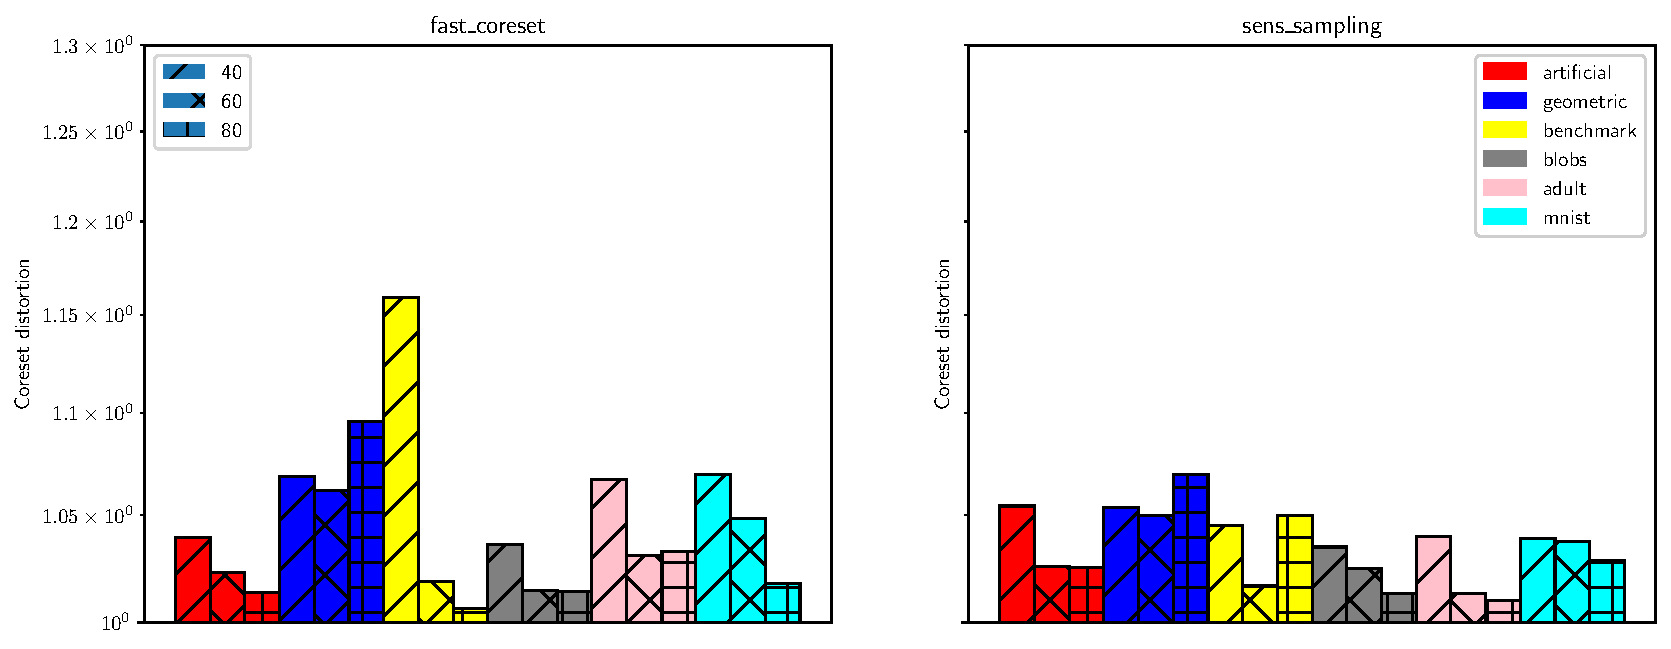
\includegraphics[width=.95\linewidth]{images/1/coreset_distortion-m_scalar_for_sens_sampling.pdf} \\

    \rotatebox[origin=l]{90}{\bf \;\;\quad\quad\quad\quad\quad\quad\quad$k$-Means} &
    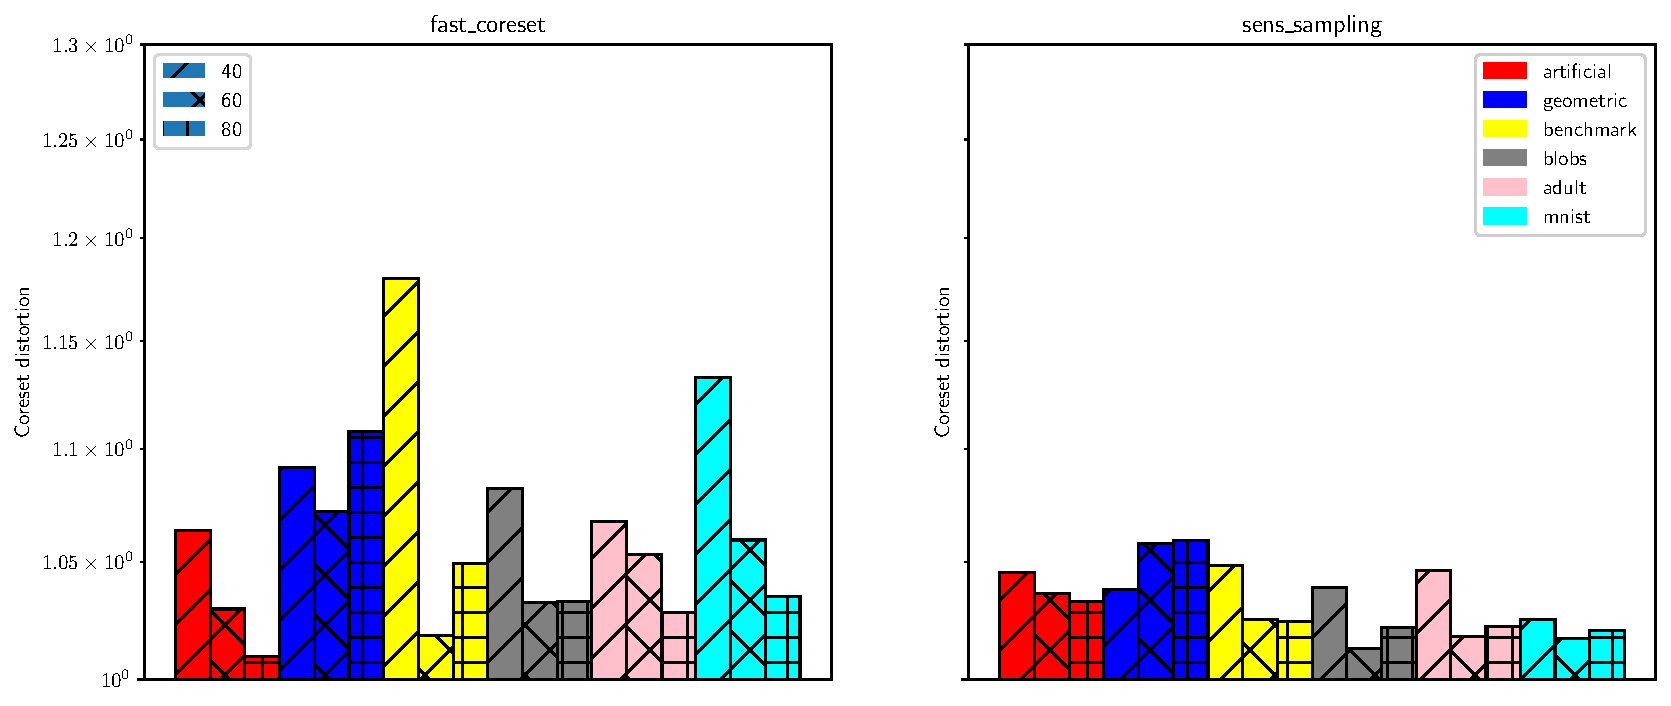
\includegraphics[width=.95\linewidth]{images/2/coreset_distortion-m_scalar_for_sens_sampling.pdf}
\end{tabular}
\caption{The effect of the coreset size on the distortion metric for sensitivity sampling approaches.
We point out that all distortion values are well below $\varepsilon = 0.2$.
Thus, for sufficient coreset sizes, there does not seem to be a meaningful difference between using Fast-Kmeans++ vs. regular Kmeans++.}
\end{figure*}


\paragraph*{Other Coreset Strategies}
\label{ssec:clustering_prelim}

Much of the advancements regarding coresets have sought the smallest coreset possible across metric spaces and downstream objectives. The most prominent
examples are in Euclidean space \cite{BadoiuHI02, HaM04, Chen09, HuangV20, stoc22}, with much of the focus on obtaining the optimal size in the $k$-means and
$k$-median setting. Recently, a lower bound \cite{huangLB} showed that the group sampling algorithm developed in \cite{stoc21, stoc22} is optimal.

Although this algorithm's coresets have size $\tilde{O}(k\cdot \varepsilon^{-2} \min(k^{z/(z+2)},\varepsilon^{-z}))$ \cite{CLSSS22} are theoretically smaller than
those obtained by sensitivity sampling, the experiments of \cite{chrisESA} showed that the latter is often more efficient in practice. We also note that one
could use virtually any coreset construction as many are linear-time once provided with an initial solution $\calC$ and assignment $\sigma$.

In terms of other linear-time methods, we are only aware of the lightweight coresets approach\cite{BachemL018}, wherein one performs sensitivity
sampling with respect to a solution $\calC=\{\mu\}$, i.e. the mean of the data set. This runs in $O(nd)$ time but provides a weaker guarantee -- one incurs an
additive error of $\varepsilon\cdot \cost(P,\{\mu\})$.  We note that this can be generalized to performing sensitivity sampling using a $\calC$ that has fewer
than $k$ centers. Since the lightweight coreset construction uses the $1$-means solution and sensitivity sampling uses an $O(1)$ approximation to the
$k$-means/median solution, it is natural to investigate the relationship between the approximation quality and coreset quality. We discuss this in more depth in
Section \ref{ssec:algorithms}.

All efficient coreset constructions are probabilistic. This comes with a disadvantage of coresets being difficult to evaluate. For example, it is co-NP-hard to
check whether a candidate compression is a weak coreset \footnote{A weak coreset guarantee only requires that a $(1+\varepsilon)$ approximation
computed on the coreset yields a $(1+\varepsilon)$ on the entire point set \cite{chrisESA}.}. Therefore, although coreset algorithms succeed with some high probability, it is
unclear how to computationally verify this.  This has posed a considerable difficulty for previous experimental evaluations and researchers would typically
focus on the cost of a solution computed on the coreset instead. We refer to \cite{chrisESA} for further discussion on this topic and discuss our metrics in
Section \ref{sssec:metrics}.

\paragraph*{Quadtree Embeddings}

To design fast algorithms, one of the common technique is to embed the Euclidean space into a tree metric.
We give a brief description of the quadtree metric embedding procedure here and refer to \cref{app:quadtree} for a more formal explanation.  The central idea is
that each hypercube in the input space can be split into $2^d$ sub-cubes and that this can be represented in a tree structure. Setting the weight of each branch
equal to the length of the parent node's diagonal then guarantees that the expected distance in the tree is within a factor $O(\log n \sqrt{d} \log
\Delta)$ of the distance in the original space,
where $\log \Delta$ is the maximum depth of the tree. Lastly, this tree can be constructed in $\tilde{O}(nd \log \Delta)$ time.

%
\subsection{Related Work.}
\david{I would put that in the intro rather than in the prelim}

The coreset paradigm has attracted a lot of attention, with a long line of work trying to get the smallest coreset possible in many different metric spaces. The
most prominent example is for Euclidean space \cite{BadoiuHI02, HaM04, Chen09, HuangV20, stoc22}.  In this case, the \textit{group sampling} algorithm developed
in \cite{stoc21, stoc22} yields a coreset of size $\tilde{O}(k\cdot \varepsilon^{-2} \min(k^{z/(z+2)},\varepsilon^{-z}))$ \cite{CLSSS22}, while we know that any
coreset must have size $\Omega \lpar k\eps^{-2}\rpar$ \cite{stoc22}.  Although group sampling has theoretically better bounds than sensitivity sampling, the
experiments of \cite{chrisESA} showed that the later one is likely to be more efficient in practice.

Small size coresets for $k$-median and $k$-means also exist in doubling metrics \cite{huang2018varepsilon}, discrete metrics \cite{FeldmanL11}, metrics induced
by minor-free graphs \cite{BravermanJKW21} or graphs with bounded treewidth \cite{baker2020coresets}.  In finite metrics, the running time $\Omega(nk)$ is
required to compute any approximation to $k$-median or $k$-means \cite{mettu2004optimal}. Since coresets can be used to quickly compute an approximation, the
running time also applies to coreset construction. 

All efficient coreset constructions are probabilistic. This comes with a disadvantage of coresets being difficult to verify and compare. For example, it is
co-NP-hard to check whether a candidate compression is a weak coreset \cite{chrisESA} \footnote{A weak coreset guarantee only requires that a $(1+\varepsilon)$
approximation computed on the coreset yields a $(1+\varepsilon)$ on the entire point set.}. Therefore, although the algorithm succeed with some high
probability, it is unknown how to determine whether the algorithm succeeded or not.  This posed a considerable difficulty for previous experimental evaluations,
where researchers would typically focus on the cost of a solution computed on the designated coreset instead.
%A recent work proposed a pipeline for doing so, and showed that sensitivity sampling algorithm slightly outperforms the theoretically best group sampling
%\cite{chrisESA}.  We will use this pipeline to evaluate the quality of the coresets analyzed in this paper.  We will use a similar heuristic to compo


\section{Coreset Algorithms}
\label{sec:theory}

In this section, we first combine two existing results to produce a strong coreset in time $\tilde{O}(nd \log \Delta)$, where $\Delta$ is the aspect-ratio of
the input.  We show afterwards how to reduce the dependency in $\Delta$ to $\log \log \Delta$, giving the desired nearly-linear runtime.

Our method is based on the following observations about the group sampling \cite{stoc21} and sensitivity sampling \cite{FeldmanL11} coreset construction
algorithms. Both start by computing a solution $\calC$. When $\calC$ is a $c$-approximation, they compute a $c \eps$-coreset of size $\tilde O\lpar
k \eps^{-z-2}\rpar$ and $\tilde O\lpar k \eps^{-2z -2}\rpar$, respectively. Hence, by rescaling, they provide $\eps$-coreset with size $\tilde O\lpar
k (\eps/c)^{-z-2}\rpar$ and $\tilde O\lpar k (\eps/c)^{-2z-2}\rpar$. 

This leads to the following fact:
\begin{fact}\label{fact:logApprox}
Let $\calC$ be an $O\lpar \log^{O(1)} k\rpar$ approximation to $k$-median or $k$-means.
Then, group sampling using solution $\calC$ computes a coreset of size $\tilde O\lpar
k \eps^{-z-2}\rpar$, and sensitivity sampling one of size $\tilde O\lpar k \eps^{-2z-2}\rpar$. 
Both runs in time $\tilde O(nd)$, provided $\calC$.
\end{fact}

To turn \cref{fact:logApprox} into an algorithm, we use the \fkmeans approximation algorithm from \cite{cohen2020fast}, which has the two following key properties: 
\begin{itemize}
\item \fkmeans runs in $\tilde O\lpar n d \log \Delta\rpar$ time (Corollary 4.3 in \cite{cohen2020fast}), and
\item \fkmeans computes an assignment from input point to centers that is a $O\lpar d^z \log k\rpar$ approximation to $k$-median ($z=1$) and
$k$-means ($z=2$) (Lemma 3.1 in \cite{cohen2020fast} for $z=2$, the discussion above for $z=1$). Applying dimension reduction techniques \cite{MakarychevMR19}, the dimension $d$ may be replaced by a $\log k$. This results in a $O\lpar\log^{z+1} k\rpar$ approximation.
\end{itemize}

The second property is crucial for us: the algorithm does not only compute centers, but also assignments in $\tilde{O}(nd\log \Delta)$ time.  We use it, in
combination with sensitivity sampling, as described in \cref{alg:main}.  This algorithm computes an $\eps$-coreset in time $\tilde O(nd \log \Delta)$: we prove
formally the statement in \cref{app:theory} Thus, it is easy to combine existing results to obtain an $\eps$-coreset without an $\tilde{O}(nk)$ time-dependency.
However, our method thus far has only replaced the $\tilde{O}(nd + nk)$ with an $\tilde{O}(nd \log \Delta)$. Indeed, the spirit of the issue remains -- this is
not log-linear in the input dimension.  We verify this in Table \ref{tbl:logdelta}, where the runtime grows linearly with the ratio of the maximum and minimum
distance.

\begin{algorithm}[tb]
   \caption{Fast-Coreset($P, k, \eps, S$)}
   \label{alg:main}
\begin{algorithmic}[1]
   \State {\bfseries Input:} data $P$, number of clusters $k$, precision $\eps$ and target size $S$
   \State Use Johnson-Lindenstrauss embedding to compute the embedding $\tilde P$ of $P$ into $\tilde d = O(\log k)$ dimensions
   \State Compute an approximate solution $\tilde \calC = \lbra \tilde c_1, ..., \tilde c_k\rbra $ for $\tilde P$, and an assignment $\tilde \sigma : \tilde P \rightarrow \tilde \calC$ using \fkmeans.	
   \State Let $\calC_i = \tilde \sigma^{-1}(c_i)$. Compute the $1$-median (or $1$-mean) $c_i$ of each $\calC_i$ in $\R^d$.%, and define $\sigma(p) := c_i$ for all $p \in \calC_i$.
   \State For each point $p \in \calC_i$, define
   $s(p) = \frac{\dist^z(p, c_i)}{\cost(\calC_i, c_i)}+ \frac{1}{|\calC_i|}$.
   \State Compute a set $\coreset$ of $S$ points randomly sampled from $P$ proportionate to $s$.
   \State For each $\calC_i$, define $|\hat \calC_i|$ the estimated weight of $\calC_i$ by $\coreset$, namely $|\hat \calC_i| := \sum_{p \in \calC_i \cap \coreset} \frac{\sum_{p' \in P}s(p')}{s(p)S}$.
   \State {\bfseries Output:} the coreset $\coreset$, with weights $w(p) = \frac{\sum_{p' \in P}s(p')}{s(p)S} \lpar (1+\eps)|\calC_i| - |\hat \calC_i|\rpar$
\end{algorithmic}
\end{algorithm}

\begin{table}[htbp]
    \centering
    \begin{tabular}{lrrrr}
        \hline
        Value of $r$ & 20 & 30 & 40 & 50 \\
        Runtime (s) & 13.5 & 14.3 & 15.7 & 16.1 \\
        \hline
        \vspace*{0.1cm}
    \end{tabular}
    \caption{Mean runtime in seconds of the \fkmeans algorithm as a function of $r$ on the $\log \Delta$-testbed dataset described in Section
    \ref{sssec:datasets}. The mean is taken over 5 runs.  Since $\log \Delta$ grows linearly with $r$, this evidences that \fkmeans indeed has a linear
    time-dependency on $\log \Delta$.}
    \label{tbl:logdelta}
\end{table}

\section{Reducing the Impact of the Spread}
\newcommand{\boxsize}{\textsc{MaxDist}}

It is well known that, for $k$-median, embedding the input into a tree using the quadtree decomposition loses only an $O(d \log \Delta)$ factor but that
building this embedding takes time $O(nd \log \Delta)$. However, we will show that we only need to build a fraction of it, allowing for a running time $O(nd
\log \log \Delta)$. 

We preface the discussion by giving an overview of the quadtree embedding algorithm. First, obtain a box enclosing all input points, centered at zero, with all
side length equal to $\boxsize$.\footnote{This can be done as follows: select an arbitrary input point, and translate the dataset so that this point is at the
origin. Then, compute the maximum distance from any point to the origin in time $O(nd)$, and let $\boxsize$ be that distance.} Then, a random shift $s \leq
\boxsize$ is added to all coordinates of all points: the input is now in the box $[-2\boxsize, 2\boxsize]^d$ and this transformation did not change any
distances, henceforth the $k$-median cost is preserved.  The $i$-th level of the tree (for $i \in \lbra 0, ..., \log \Delta \rbra$) is constructed as follows:
a grid of side length $2^{-i} \cdot 2\boxsize$ centered at $0$ is placed, and each cell is a node in the tree.  The parent of a cell $c$ is simply the cell at
level $i-1$ that contains $c$, and the distance between $c$ and its parent is set to $\sqrt{d}2^{-i} \cdot 2\boxsize$ (namely, the $\ell_2$ diameter of $c$).
 
This tree has $O(\log \Delta)$ levels, and it is known that for any solution $\calS$, its cost in the tree metric is within a factor $O(\sqrt d \log \Delta)$ of
its cost for the original metric. Therefore, it is enough for us to find an approximation in the tree metric. We let $\opt_T$ be the optimal solution in the
tree metric, bounded as follows:
 
To remove the $\log\Delta$ dependency, we proceed in two steps: first, we compute a very crude upper-bound on the cost $U$ of the optimal
solution -- up to a $\poly(n)$ factor.  If $U$ is a $c$-approximation of the optimal cost, the natural attempt to reduce the aspect-ratio is to round all
coordinates to multiples of $g = U/(cn)$, giving us a minimum distance of $g$; it is then enough to reduce the diameter to $\poly(n) U$. We proceed as
follows: we place a grid with cell length $O(n \cdot U)$, so that two points from the same cluster in $\opt$ fall into the same cell w.h.p. That way, the
distinct cells do not interact with each other in any reasonable solution.  Then, we compress the input by "moving" non-empty cells closer to each other.

\subsection{Computing a crude upper-bound}

As described, we start by computing an approximate solution $U$ such that $U \leq \poly(n) \cdot \cost(\opt)$ on an.  We focus here on the simpler $k$-median
problem, and show in \cref{app:redKM} how to reduce $k$-means to this case. Our first step is embedding the input into a quadtree as described above. In this
tree, our first lemma shows the necessary approximation exists at the first level for which the input lies in $k+1$ disjoint subtrees. The algorithm to find
this is then a simple binary search through the levels of the tree.

\begin{lemma}\label{lem:apxTree}
Let $i$ be the first level of the decomposition such that at least $k+1$ cells at level $i$ contains any point. Then, $\sqrt{d}2^{-i+1} \cdot \boxsize \leq
\opt_T \leq n \cdot \sqrt{d}2^{-i+4} \cdot \boxsize$.
\end{lemma}

We prove this in Section \ref{app:apx-tree-proof} of the appendix. A direct consequence of this lemma is that the first level of the tree for which at least
$k+1$ cells are non empty provides an $O(n)$-approximation. To count the number of non-empty cells at a given level $i$, one can merely iterate over all
points, for each point identify the cell that contains it (using modulo operation), and store all those cells into a hash table to count the number of elements.
This is done in time $O(nd)$.  Using a binary search on the $O(\log \Delta)$ many levels then concludes this section with the following result:

\begin{lemma}\label{lem:crudeApx}
There is an algorithm running in time $O(nd \log \log \Delta)$ that computes an  $O(n^2 d \log \Delta)$-approximation to $k$-median or $k$-means.
\end{lemma}

\subsection{From Approximate Solution to Small Aspect-Ratio}
Let $U$ be an upper-bound on the optimal cost that is a $c$-approximation, computed via \cref{lem:crudeApx}. We place a grid with side length $d n^2\cdot U$.
The following folklore lemma ensures that with high probability, no cluster of the optimal solution is spread on several grid cells.

\begin{lemma}
The probability that two points $p$ and $q$ are in different grid cells is $O\lpar \frac{\|p-q\|^2}{n^2 U}\rpar$
\end{lemma}

Since $U$ is larger than the distance between any input point and its center in the optimal solution, a union-bound ensures that with probability $1-1/n$, no
cluster of this solution is split among different cells.  In particular, there are at most $k$-non empty cells. We call those "boxes".

From this input, we build a new set of points $P'$ as follows: first, identify the non empty cell (using a hash table as previously). We associate each box with
its center.  For each coordinate $i \in \lbra 1, ..., d \rbra$, sort (in time $O(k \log k)$) the centers according to their value on coordinate $i$. Then, for
each $j \in \lbra 1, ..., k\rbra$, let $c^i_j$ and $c^i_{j+1}$ be the $i$-th coordinate of centers of the $j$-th and $(j+1)$-th boxes. If $c^i_{j+1} - c^i_j
\geq 2d n^2\cdot U$, then for all cells $j'$ with $j' > j$, shift the points of $j'$ by $c^i_{j+1} - c^i_j - 2d n^2\cdot U$ in the $i$-th coordinate.

This can be implemented with a linear scan, and has two effects: first, the diameter of the input is now $\sqrt{d} \cdot 2d n^2\cdot U \cdot k$, as along any
coordinate the maximal distance is $2d n^2\cdot U \cdot k$. Second, two boxes that were adjacent are still adjacent and two boxes that were non-adjacent are
still non-adjacent.

The first property allows us to reduce the aspect-ratio to $(nd \log \Delta)^{O(1)}$.  Indeed, one can round all coordinates to the closest multiple of
$g = \frac{U}{n^4 d^{2} \log \Delta}$. Since every point has moved by at most $g$ and, using \cref{lem:crudeApx}, $U
\leq n^2 d \log(\Delta) \opt$, it is clear that the distance between any point and its rounding is at most $\frac{\opt}{n^2}$. Summing this error over all points,
any solution computed on the gridded data has cost within an additive factor $\pm \frac{\opt}{n}$ of the true cost. Furthermore, the smallest
non-zero distance is $g = \frac{U}{n^4 d^{2} \log \Delta}$, implying that the aspect-ratio of the new metric is $(nd \log \Delta)^{O(1)}$,
as claimed.

The second property, on the other hand, ensures that we can transform a solution $\calS'$ for $P'$ to a solution with exactly the same cost for $P$: in any
(reasonable) solution, points from two non-adjacent boxes will not be in the same cluster in either $P'$ or $P$. Therefore, simply adding back the corresponding
shift to centers of $\calS'$ allows us to transform it to a solution $\calS$. We note that the distance between any point and its closest center does not
change. This is formalized in the next lemma.

\begin{lemma}
Let $\calS'$ be a $c'$-approximation for  $k$-median (resp. $k$-means) on $P'$, where $c' \leq nc$ and $c$ is the approximation guarantee from \cref{lem:crudeApx}. Then, one can compute a solution for $P$ for $k$-median (resp. $k$-means) on $P$, with same cost as $\calS'$ for $P'$, in time $O(nd)$.
\end{lemma}
\begin{proof}

First, since distances in $P'$ are smaller than in $P$, the optimal solution for $P'$ has cost at most $U$. Therefore, two points that are in non-adjacent boxes
(i.e., at distance more than $d n^2\cdot U$) are not in the same cluster of $\calS'$ -- as otherwise $\calS'$ would not be a $c'$-approximation.  Let $\calS$ be
the solution obtained from $\calS'$ by reversing the construction of $P'$. Since this construction preserves adjacency, for all clusters of the solution, all
distances are the same in $P$ and $P'$. Therefore, the costs are equal.

\end{proof}

\subsection*{Extensions.} 
We conclude this section with a few remarks that allow us to generalize \cref{alg:main}.

Consider that \cref{alg:main}  only needs to be provided with an assignment to a solution that is a $O(\polylog k)$ approximationone, implying that one could
compute the solution $\calC$ via any algorithm that satisfies this.  This initial solution may as well be an $O\lpar\polylog \lnor P \rnor_0 \rpar$
approximation: using the iterative coreset construction from \cite{BravermanJKW21}, one could then derive a near-optimal coreset size, only suffering
a $O(\log^* n)$ loss in the running time.

As an example, we illustrate a different approach for $k$-median. One could first embed the input into a hierarchically separated tree (HST) with expected
distortion $O(\log \lnor P \rnor_0)$ \cite{FakcharoenpholRT03}. On such tree metrics, solving $k$-median can be done in linear time using dedicated algorithms
(see e.g. \cite{Cohen-AddadLNSS21}). Using the solution from the HST metric, one can compute a coreset, and iterate using the previous argument.  This embedding
into HST is very similar to what is done by the \fkmeans algorithm, but can be actually performed in \emph{any} metric space, not only Euclidean.  For instance,
in a metric described by a graph with $m$ edges, the running time of this construction would be near linear-time $\tilde O(m)$.

%\section{Reducing the Impact of the Spread}
To reduce the dependency of $\Delta$ on the running time, we proceed in two steps: first, we compute a very crude upper-bound on the cost $U$ of the optimal solution -- up to a $\poly(n)$ factor. 
If $U$ is a $c$-approximation of the optimal cost, the natural attempt to reduce the aspect-ratio is to round all coordinates to multiples of $U/(cnà$, such that the smallest distance is $U/(cn)$; it is then enough to reduce the diameter to $\poly(n) U$. We proceed as follows: we place a grid with cell length $O(n \cdot U)$, so that two points from the same cluster in $\opt$ fall into the same cell w.h.p. That way, the distinct cells do not interact with each other in any reasonable solution. 
Then, we compress the input by "moving" non-empty cells closer to each other.

\subsection{Computing a crude upper-bound}
As described, we start by computing a $U$ such that $U \leq \poly(n) \cdot \cost(\opt)$. For this, we start by simplifying a lot our task: our first lemma shows that it is enough focus on the $k$-median problem; we then embed the input into a tree, easier to handle than Euclidean space. In this tree, we will show that it is enough to find the first level for which the input lies in $k+1$ disjoint subtrees: the final algorithm is therefore a mere binary-search to find efficiently this level.

\paragraph{Reduction to $k$-median.}

\begin{lemma}
Let $\calS$ be a $c$-approximation for $k$-median on $P$. Then, $\calS$ is a $nc^2$-approximation for $k$-means on $P$.
\end{lemma}
\begin{proof}
Let $\cost_1$ (resp. $\cost_2$) be the $k$-median (resp. $k$-means) cost, $\opt_1$ (resp. $\opt_2$) be the optimal $k$-median (resp. $k$-means) solution. We have the following inequalities:
\begin{align*}
\cost_2(\calS) &= \sum_{p\in P} \dist(p, \calS)^2 \leq \lpar \sum_{p\in P} \dist(p, \calS)\rpar^2\\
&\leq c^2 \cdot \lpar  \sum_{p\in P} \dist(p, \opt_1)\rpar^2\\
&\leq c^2 \cdot \lpar  \sum_{p\in P} \dist(p, \opt_2)\rpar^2\\
&\leq c^2 \cdot n \cdot  \sum_{p\in P} \dist(p, \opt_2)^2,
\end{align*}
where the last inequality stems from Cauchy-Schwarz. Therefore, $\calS$ is a $nc^2$ - approximation to $k$-means. 
\end{proof}

\paragraph{Reduction to Structured Tree.}
\newcommand{\boxsize}{\textsc{MaxDist}}
It is well known that, for $k$-median, embedding the input into a tree using the quadtree decomposition loses only a $O(d \log \Delta)$ factor. Building explicitely this embedding takes time $O(nd \log \Delta)$: however, we will show that we only need to build only a fraction of it, allowing for a running time $O(nd \log \log \Delta)$. 

The embedding is constructed as follows. First, the algorithm finds a box enclosing all input points, centered at zero, with all side length equal to $\boxSize$.\footnote{This can be done as follows: select an arbitrary input point, and translate the dataset so that this point is at the origin. Then, compute the maximum distance from any point to the origin in time $O(nd)$, and let $\boxSize$ be that distance.} Then, a random shift $s \leq \boxsize$ is added to all coordinates of all points: the input is now in the box $[-2\boxsize, 2\boxsize]^d$ and this transformation did not change any distances, henceforth the $k$-median cost is preserved. 
The $i$-th level of the tree (for $i \in \lbra 0, ..., \log \Delta \rbra$) is constructed as follows: a grid of side length $2^{-i} \cdot 2\boxsize$ centered at $0$ is placed, and each cell is a node in the tree.
 The parent of a cell $c$ is simply the cell at level $i-1$ that contains $c$, and the distance between $c$ and its parent is set to $\sqrt{d}2^{-i} \cdot 2\boxsize$ (namely, the $\ell_2$ diameter of $c$).
 
 This tree has $O(\log \Delta)$ levels, and it is known that for any solution $\calS$, its cost in the tree metric is within a factor $O(\sqrt d \log \Delta)$ of its cost for the original metric. Therefore, it is enough for us to find an approximation in the tree metric. For this, we let $\opt_T$ be the optimal solution in the tree metric, and have the following lemma:
 
\begin{lemma}\label{lem:apxTree}
Let $i$ be the first level of the decomposition such that at least $k+1$ cells at level $i$ contains any point. Then, $\sqrt{d}2^{-i+1} \cdot \boxsize \leq \opt_T \leq n \cdot \sqrt{d}2^{-i+4} \cdot \boxsize$.
\end{lemma}
\begin{proof}
If the input is spread in $k+1$ distinct cell at level $i$, then in any solution there is at least one of those cells with no center. In the tree metric, points lying in this cell have therefore connexion cost at least $\sqrt{d}2^{-i+1} \cdot \boxsize$, and thus the left-hand-side of the inequality holds.

On the other hand, if the input is contained into $k$ cells at level $i-1$, then placing arbitrarily a center in each cell yields a solution with cost at most $n \cdot \sqrt{d}2^{-i+4} \cdot \boxsize$: indeed, the distance from any point to its closest center is at most $2 \cdot \sum_{j \geq i-1} \sqrt{d}2^{-j} \cdot 2\boxsize \leq 4 \sqrt{d}2^{-i+2} \cdot \boxsize$ (summing the edge length from the point to the cell at level $i$, and then going down to the center). This concludes.
\end{proof}

A consequence of \cref{lem:apxTree} is that the first level of the tree for which at least $k+1$ cells are non empty provides an $O(n)$-approximation. 
To count the number of non-empty cells at a given level $i$, one can merely iterate over all points, for each point identify the cell that contains it (using modulo operation), and store all those cells into a hash table to count the number of elements. This is done in time $O(nd)$.
Using a binary search on the $O(\log \Delta)$ many levels then concludes this section with the following result:

\begin{lemma}\label{lem:crudeApx}
There is an algorithm running in time $O(nd \log \log \Delta)$ that computes an  $O(n^2 d \log \Delta)$-approximation to $k$-median or $k$-means.
\end{lemma}

\subsection{From Approximate Solution to Small Aspect-Ratio}
Let $U$ be an upper-bound on the optimal cost that is a $c$-approximation, computed via \cref{lem:crudeApx}. We place a grid with side length $d n^2\cdot U$.
The following folklore lemma ensures that with high probability, no cluster of the optimal solution is spread on several grid cells.

\begin{lemma}
The probability that two points $p$ and $q$ are in different grid cells is $O(\frac{\|p-q\|^2}{n^2 U}$
\end{lemma}
Since $U$ is larger than the distance between any input point and its center in the optimal solution, a union-bound ensures that with probability $1-1/n$, no cluster of this solution is split among different cells.
In particular, there are at most $k$-non empty cells. We call those "boxes".

From this input, we build a new one $P'$ as follows: first, identify the non empty cell (using a hash table as previously). We associate each box with its center.
For each coordinate $i \in \lbra 1, ..., d \rbra$, sort (in time $O(k \log k)$ the centers according to their value on coordinate $i$. Then, for each $j \in \lbra 1, ..., k\rbra$, let $c^i_j$ and $c^i_{j+1}$ be the $i$-th coordinate of centers of the $j$-th and $(j+1)$-th boxes. If $c^i_{j+1} - c^i_j \geq 2d n^2\cdot U$, then for all cell $j'$ with $j' > j$, shift points  of $j'^$ by an amount $c^i_{j+1} - c^i_j - 2d n^2\cdot U$ in $i$-th coordinate.


This can be implemented with a linear scan, and has two effects: first, the diameter of the input is now $\sqrt{d} \cdot 2d n^2\cdot U \cdot k$, as along any coordinate the maximal distance is $2d n^2\cdot U \cdot k$. Second, two boxes that were adjacents are still adjacents, and two boxes that were non-adjacents are still non-adjacent.

The first property allows to reduce the spread to $(nd \log \Delta)^{O(1)}$. Indeed, one can round all coordinates to the closest multiple of $\frac{U}{n^4 d^{2} \log \Delta}$. That way, each point is at distance at most $\frac{U}{n^4 d^{2} \log \Delta}$ of its rounding. using \cref{lem:crudeApx}, $U \leq n^2 d \log(\Delta) \opt$, and therefore the distance between any point and its rounding is at most $\frac{\opt}{n^2}$. Summing this error over all points, this ensures that any solution computed on the rounding has cost within an additive factor $\pm \frac{\opt}{n}$ of the true cost. Furthermore, the smallest non-zero distance is $\frac{U}{n^4 d^{2} \log \Delta}$, and therefore the spread of the new metric is $2 n^6 d k \log \Delta = (nd \log \Delta)^{O(1)}$, as claimed.

The second property, on the other hand, ensures that we can transform a solution $\calS'$ for $P'$ to a solution with exactly the same cost for $P$: in any (reasonable) solution, points from two non-adjacent box will not be in the same cluster in $P'$ nor in $P$. Therefore, simply adding to centers of $\calS'$ the corresponding shift allows to transform it to a solution $\calS$, such that the distance between any point and its closest center does not change. This is formalized in the next lemma.

\begin{lemma}
Let $\calS'$ be a $c'$-approximation for  $k$-median (resp. $k$-means) on $P'$, where $c' \leq nc$ and $c$ is the approximation guarantee from \cref{lem:crudeApx}. Then, one can compute a solution for $P$ for $k$-median (resp. $k$-means) on $P$, with same cost as $\calS'$ for $P'$, in time $O(nd)$.
\end{lemma}
\begin{proof}
First, since distances in $P'$ are smaller than in $P$, the optimal solution for $P'$ has cost at most $U$. Therefore, two points that are in non-adjacent boxes (i.e., at distance more than $d n^2\cdot U$) are not in the same cluster of $\calS'$ -- as otherwise $\calS'$ would not be a $c'$-approximation.

Let $\calS$ be the solution obtained from $\calS'$ by reversing the construction of $P'$. Since this construction preserves adjacency, for all cluster of the solution, all distances are the same in $P$ and $P'$: therefore, the cost are alike. This concludes.
\end{proof}


\section{Fast Compression in Practice}
\label{sec:results}

Despite the near-linear time algorithm described in Sections~\ref{sec:theory_0} and~\ref{sec:theory}, the coreset construction of \cref{alg:main} nonetheless
requires a bounded approximation to the original task before the sampling can occur. Although theoretically justified, it is unclear how necessary this is in
practice -- would a worse approximation factor still be representative of the dataset for practical purposes? We answer this question by defining a suite of
algorithms, datasets and evaluation procedures that allow for a comprehensive study of speed vs. accuracy tradeoffs in compression for clustering.  We begin by
describing our experimental setup before showing results in both the static and streaming settings. We note that these results correspond directly to
downstream clustering tasks. Unless stated otherwise, our experimental results focus on the $k$-means task.

\subsection{Experimental Setup}
\paragraph*{Metrics}
\label{sssec:metrics}

We analyze the sampling methods along two metrics -- compression accuracy and construction time. Although measuring runtime is standard, it is unclear how to
confirm that a subset of points satisfies the coreset property over all solutions. To this end, we use the distortion measure introduced in~\cite{chrisESA} $
\max \left( \dfrac{\cost(P, \calC_{\Omega})}{\cost(\Omega, \calC_{\Omega})}, \dfrac{\cost(\Omega, \calC_{\Omega})}{\cost(P, \calC_{\Omega})} \right),$ where
$\calC_{\Omega}$ is a candidate solution computed over the coreset $\Omega$. This will be within $1+\varepsilon$ if the coreset guarantee is satisfied
but may be unbounded otherwise.  We refer to this as the \emph{coreset distortion}.

\begin{table}
    \centering
    \begin{tabular}{lrr}
        Dataset & Points & Dim \\
        \hline
        \emph{Adult} & 48\,842 & 14 \\
        \emph{MNIST} & 60\,000 & 784 \\
        \emph{Song} & 515\,345 & 90 \\
        \emph{Cover Type} & 581\,012 & 54 \\
        \emph{Census} & 2\,458\,285 & 68 \\
        \hline
    \end{tabular}
    \caption{Description of real world datasets}
    \label{tbl:datasets}
\end{table}


\paragraph*{Algorithms}
\label{ssec:algorithms}

We compare Fast-Coresets (Algorithm~\ref{alg:main}) against 5 different benchmark sampling strategies that span the space between optimal time and optimal
accuracy.
\begin{description}
        \item \emph{- Standard uniform sampling}. Each point is sampled with equal probability and weights are set to $n / m$, where $m$ is the size of the sample.
        \item \emph{- Standard sensitivity sampling \cite{LS10}}. We refer to Section~\ref{sec:preliminaries}.
        \item \emph{- Lightweight coresets \cite{bachem2018scalable}}. Obtain a coreset by sampling sensitivity values with respect to the $1$-means solution,
            i.e. sensitivities are given by $\hat{s}(p) = 1/|P| + \cost(p, \mu) / \cost(P, \mu)$, where $\mu$ is the dataset mean.
        \item \emph{- Welterweight coresets}. For any $j \in \{1,..., k\}$, we compute a coreset using sensitivity sampling with respect to a candidate
            $j$-means solution.
        \item \emph{- BICO \cite{bico}}. Utilizes BIRCH \cite{birch} to produce a $k$-means coreset in a stream.
\end{description}

\begin{table*}
    \centering
    \vspace*{-0.1cm}
    \tiny
    \begin{tabular}{|c|cc|cc|cc|cc|}
        \hline
        & \multicolumn{8}{c|}{Method} \\
        \cline{2-9} & \multicolumn{2}{c|}{Uniform Sampling} & \multicolumn{2}{c|}{Lightweight} & \multicolumn{2}{c|}{Welterweight} & \multicolumn{2}{c|}{Fast Coreset} \\
        & $m=40k$ & $m=80k$ & $m=40k$ & $m=80k$ & $m=40k$ & $m=80k$ & $m=40k$ & $m=80k$ \\
        \cline{2-9}
        $c$-outlier & 405 $\pm$ 24K & 159 $\pm$ 20K & 1.07 $\pm$ 0.0 & 5.63 $\pm$ 84.6 & 9.44 $\pm$ 105 & 1.03 $\pm$ 0.0 & 1.12 $\pm$ 0.0 & 1.05 $\pm$ 0.0 \\
        Geometric & 86.3 $\pm$ 8.4K & 21.8 $\pm$ 652 & 1.05 $\pm$ 0.0 & 11.6 $\pm$ 452 & 1.11 $\pm$ 0.0 & 1.03 $\pm$ 0.0 & 1.11 $\pm$ 0.0 & 1.05 $\pm$ 0.0 \\
        Gaussian Mix. & 3.17 $\pm$ 3.42 & 1.43 $\pm$ 0.25 & 2.64 $\pm$ 1.61 & 1.81 $\pm$ 0.58 & 2.26 $\pm$ 1.55 & 1.28 $\pm$ 0.07 & 1.24 $\pm$ 0.0 & 1.13 $\pm$
        0.0 \\
        \makecell{Benchmark\\---} & \makecell{1.07 $\pm$ 0.0\\---} & \makecell{1.03 $\pm$ 0.0\\---} & \makecell{1.11 $\pm$ 0.0\\---} & \makecell{1.05 $\pm$
        0.0\\---} & \makecell{1.10 $\pm$ 0.0\\---} & \makecell{1.04 $\pm$ 0.0\\---} & \makecell{1.15 $\pm$ 0.0\\---} & \makecell{1.06 $\pm$ 0.0\\---} \\
        MNIST & 1.08 $\pm$ 0.0 & 1.03 $\pm$ 0.0 & 1.08 $\pm$ 0.0 & 1.03 $\pm$ 0.0 & 1.08 $\pm$ 0.0 & 1.04 $\pm$ 0.0 & 1.08 $\pm$ 0.0 & 1.04 $\pm$ 0.0 \\
        Adult & 1.08 $\pm$ 0.0 & 1.04 $\pm$ 0.0 & 1.09 $\pm$ 0.0 & 1.04 $\pm$ 0.0 & 1.32 $\pm$ 0.0 & 1.17 $\pm$ 0.0 & 1.17 $\pm$ 0.0 & 1.07 $\pm$ 0.0 \\
        Song & 1.30 $\pm$ 0.0 & 1.14 $\pm$ 0.0 & 1.13 $\pm$ 0.0 & 1.12 $\pm$ 0.0 & 1.18 $\pm$ 0.0 & 1.16 $\pm$ 0.0 & 1.50 $\pm$ 0.0 & 1.29 $\pm$ 0.0 \\
        Census & 1.15 $\pm$ 0.0 & 1.07 $\pm$ 0.0 & 1.12 $\pm$ 0.0 & 1.06 $\pm$ 0.0 & 1.14 $\pm$ 0.0 & 1.06 $\pm$ 0.0 & 1.13 $\pm$ 0.0 & 1.07 $\pm$ 0.0 \\
        Cover-Type & 1.12 $\pm$ 0.0 & 1.05 $\pm$ 0.0 & 1.11 $\pm$ 0.0 & 1.06 $\pm$ 0.0 & 1.17 $\pm$ 0.0 & 1.08 $\pm$ 0.0 & 1.11 $\pm$ 0.0 & 1.04 $\pm$ 0.0 \\
        \hline
    \end{tabular}
    \caption{Distortion means and variances for different sample sizes across datasets; taken over 5 runs.}
    \label{tbl:distortion}
    \vspace*{0.1cm}
    \tiny
    \begin{tabular}{|c|cc|cc|cc|cc|}
        \hline
        & \multicolumn{8}{c|}{Method} \\
        \cline{2-9} & \multicolumn{2}{c|}{Uniform Sampling} & \multicolumn{2}{c|}{Lightweight} & \multicolumn{2}{c|}{Welterweight} & \multicolumn{2}{c|}{Fast Coreset} \\
        & Streaming & Static & Streaming & Static & Streaming & Static & Streaming & Static \\
        \cline{2-9}
        $c$-outlier & 221 $\pm$ 15K & 261 $\pm$ 44K & 1.07 $\pm$ 0.0 & 5.51 $\pm$ 78.9 & 1.09 $\pm$ 0.0 & 12.1 $\pm$ 80.1 & 1.13 $\pm$ 0.0 & 1.11 $\pm$
        0.0 \\
        Geometric & 66.5 $\pm$ 2.7K & 140 $\pm$ 1.8K & 85.2 $\pm$ 2.8K & 45.6 $\pm$ 4.2K & 1.09 $\pm$ 0.0 & 10.4 $\pm$ 349 & 1.15 $\pm$ 0.0 & 1.12 $\pm$ 0.0 \\
        Gaussian Mix. & 1.51 $\pm$ 0.07 & 2.42 $\pm$ 2.52 & 2.35 $\pm$ 0.67 & 2.38 $\pm$ 1.78 & 1.45 $\pm$ 0.05 & 3.65 $\pm$ 3.85 & 1.15 $\pm$ 0.0 & 1.24 $\pm$
        0.0 \\
        Benchmark & 1.10 $\pm$ 0.0 & 1.07 $\pm$ 0.0 & 1.08 $\pm$ 0.0 & 1.11 $\pm$ 0.0 & 1.09 $\pm$ 0.0 & 1.11 $\pm$ 0.0 & 1.18 $\pm$ 0.0 & 1.16 $\pm$ 0.0 \\
        MNIST & 1.42 $\pm$ 0.0 & 1.08 $\pm$ 0.0 & 1.07 $\pm$ 0.0 & 1.07 $\pm$ 0.0 & 1.02 $\pm$ 0.0 & 1.09 $\pm$ 0.0 & 1.12 $\pm$ 0.0 & 1.08 $\pm$ 0.0 \\
        Adult & 1.33 $\pm$ 0.0 & 895K $\pm$ 3.2B & 1.09 $\pm$ 0.0 & 1.09 $\pm$ 0.0 & 1.27 $\pm$ 0.01 & 1.32 $\pm$ 0.0 & 1.14 $\pm$ 0.0 & 1.15 $\pm$ 0.0 \\
        \hline
    \end{tabular}
    \caption{Distortion means and variances in the streaming and non-streaming setting for each method.}
    \label{tbl:composition}
\end{table*}



We use $j$ going forward to describe the number of solutions in the candidate $j$-means solution. Thus, lightweight coresets have $j=1$ while Fast-Coresets have
$j=k$.

We take a moment here to motivate the welterweight coreset algorithm.  Consider that lightweight coresets use the $1$-means solution to obtain the sensitivities
that dictate the sampling distribution. On the other hand, sensitivity sampling is solving the full $k$-means problem. Thus, changing the value of $j$ affects
the cluster sizes $|\calC_p|$ and therefore acts as a direct interpolation between uniform and sensitivity sampling.  We default to $j = \log k$ unless stated
otherwise. We use the term `accelerated sampling methods' when referring to uniform, lightweight and welterweight coresets as a group.

\paragraph*{Datasets}
\label{sssec:datasets}

We employ several real and artificial datasets to evaluate the quality of a coreset.  For our real-world data, we utilize the Adult~\cite{Dua:2019},
MNIST~\cite{mnist}, Song~\cite{song}, Census~\cite{census}, and Cover Type~\cite{covtype} datasets, whose characteristics are summarized in
Table~\ref{tbl:datasets}. These are standard datasets for coreset and clustering evaluations.
We complement these with artificial datasets and default to $n = 50\,000$ and $d=50$ unless stated otherwise.
\begin{description}
    \item \emph{- c-outlier}. Place $n-c$ points in a single location and $c$ points a large distance away.
    \item \emph{- Geometric}. Place $c k$ points at $(1, 0, 0, \cdots)$, $\frac{ck}{r}$ points at $(0, 1, 0, \cdots)$, $\frac{ck}{r^2}$ points
        at $(0, 0, 1, \cdots)$, and so on for $\log_r (ck)$ rounds. Thus, the data creates a high-dimensional simplex with uneven weights across the vertices. We
        default to $c = 100$ and $r=2$.
    \item \emph{- Gaussian mixture}. A set of scattered Gaussian clusters of varying density.

        These clusters are sequentially defined, with the size of the first cluster defined by $\frac{n}{\kappa} \exp \left( \gamma \cdot \rho_0 \right)$, where
        $\kappa$ is the number of Gaussian clusters, $\rho_0$ is uniformly chosen from $[-0.5, 0.5]$, and $\gamma$ is a hyperparameter that affects the
        distribution of cluster sizes.  Then, given clusters $\{c_1, \cdots, c_i\}$, we obtain the size of the $(i+1)$-st cluster by \[ \quad \quad \quad \quad |c_{i+1}|
        = \frac{n - \sum_i |c_i|}{\kappa - i}\exp \left( \gamma \cdot \rho_{i+1} \right).\]

        This has the property that all clusters have size $n / k$ when $\gamma = 0$ and, as $\gamma$ grows, the cluster sizes diverge at an exponential rate.
        We note that this is a well-clusterable instance with respect to cost stability conditions, see \cite{AwS12,Cohen-AddadS17,KuK10,ORSS12}.

    \item \emph{- Benchmark}. A specific distribution of points introduced in \cite{chrisESA} as a testbed for coreset algorithms.  It has the property that all
        reasonable $k$-means solutions are of equal quality but are maximally far apart in the solution space. Thus, the dataset is fully determined by the
        number of centers $k$. As suggested, we produce three benchmark datasets of varying size before applying random offsets to each. We choose the sizes by
        $k_1 = \frac{k}{c_1}$, $k_2 = \frac{k - k_1}{c_2}$, and $k_3 = k - k_1 - k_2$ for $c_1, c_2 \in \mathbb{R}^+$.

\end{description}

The artificial datasets are constructed to emphasize strengths and weaknesses of the various sampling schemas. For example, the $c$-outlier problem contains
very little information and, as such, should be simple for any sampling strategy that builds a reasonable representation of its input. The geometric dataset
then increases the difficulty by having more regions of interest that must be sampled. The Gaussian mixture dataset is
harder still, as it incorporates uneven inter-cluster distances and inconsistent cluster sizes. Lastly, the benchmark dataset is devised to be a worst-case
example for sensitivity sampling.

\paragraph*{Data Parameters}
\label{app:data_params}

In all real and artificial datasets, we add random uniform noise $\eta$ with $0 \leq \eta_i \leq 0.001$ in each dimension in order to make all points unique.
Unless specifically varying these parameters, we default all algorithms in~\ref{ssec:algorithms} to $k=100$ for the Adult, MNIST, and artificial datasets and
$k=500$ for the Song, Cover Type, and Census datasets. Our default coreset size is then $m = 40k$. We refer to the coreset size scalar as the \emph{$m$-scalar}.
We only run the dimension-reduction step on the MNIST dataset, as the remaining datasets already have sufficiently low dimensionality.  We run our experiments
on an Intel Core i9 10940X 3.3GHz 14-Core processor.

\subsection{Evaluating Sampling Strategies}
\label{ssec:alg_qualities}

\paragraph*{Theoretically guaranteed methods.}

We first compare the Fast-Coreset algorithm with standard sensitivity sampling to ensure that it obtains appropriate accuracy in a shorter runtime.  To this
end, the last columns of Tables~\ref{tbl:distortion} and~\ref{tbl:composition} show that the Fast-Coreset method produces compressions of consistently low
distortion and that this holds across datasets, $m$-scalar values and in the streaming setting.  Despite this, Figure~\ref{fig:coreset_size_on_sens_quality}
shows that varying $k$ from $50$ to $400$ causes a linear slowdown in sensitivity sampling but only a logarithmic one for the Fast-Coreset method. This analysis
confirms the theory in Section~\ref{sec:theory} and we therefore do not add traditional sensitivity sampling to the other experiments.

\paragraph*{Speed vs. Accuracy.}

\begin{figure}
\centering
\begin{tabular}{lc}
    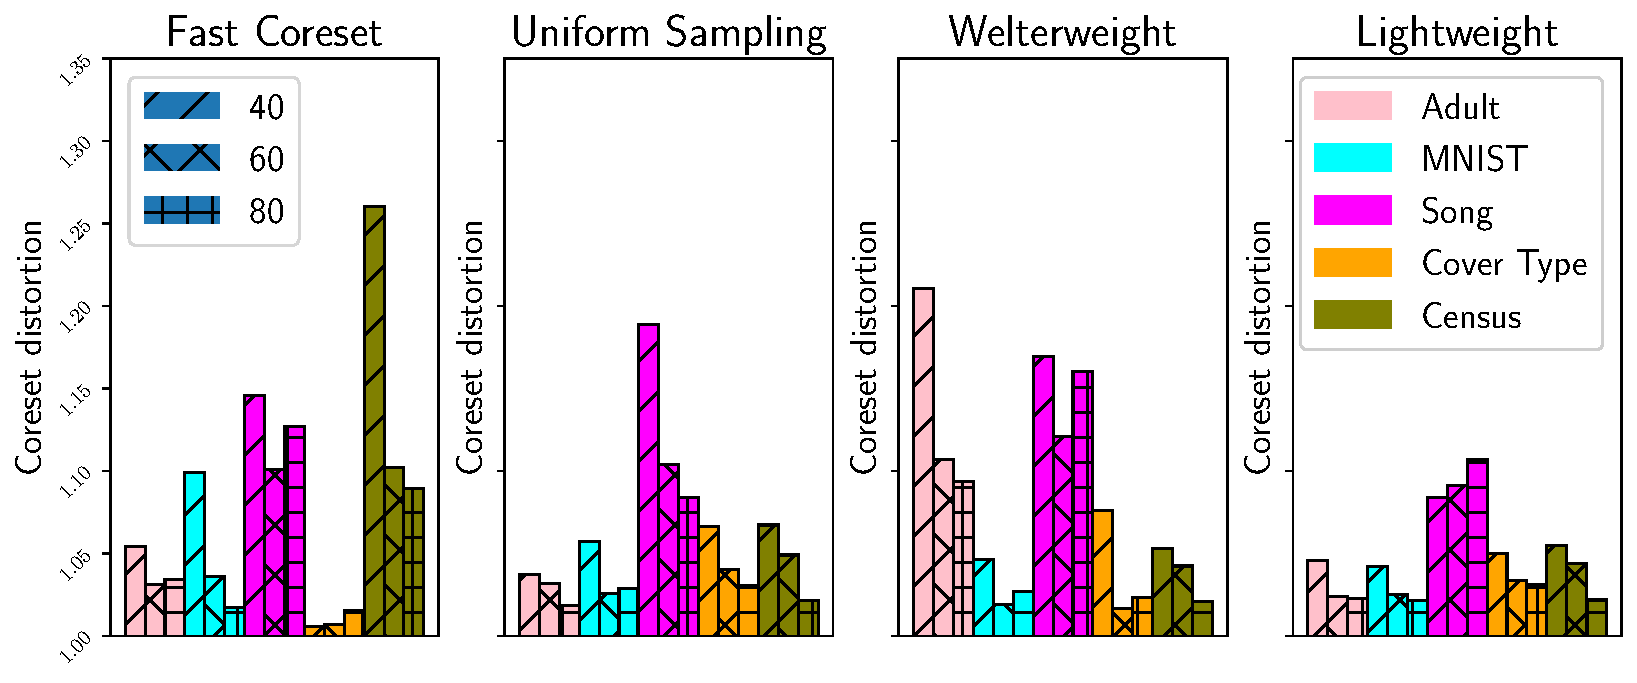
\includegraphics[width=\linewidth]{images/distortion_real_data} \\
    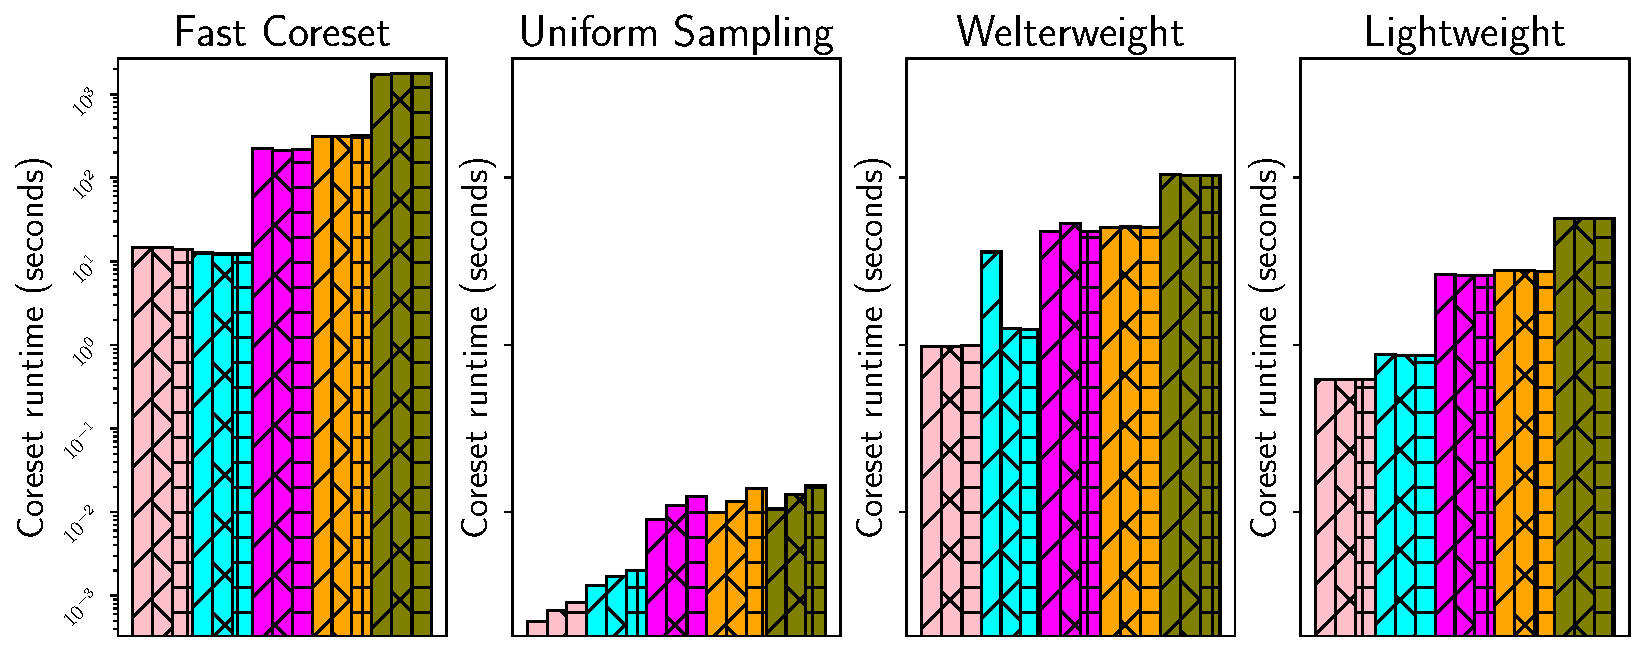
\includegraphics[width=\linewidth]{images/runtime_real_data}
\end{tabular}

\caption{\emph{Top}: The effect of the $m$-scalar on coreset distortion for real-world datasets. This is a visualization of the data in
Table~\ref{tbl:distortion}.  \emph{Bottom}: The effect of the $m$-scalar on the algorithm runtime for real-world datasets. All values are the mean over 5 runs.
The three bars represent samples of size $m=40k, 60k, 80k$.}

\label{fig:coreset_size_on_quality}
\end{figure}


We now refer the reader to the remaining columns of Table~\ref{tbl:distortion} and Figure~\ref{fig:coreset_size_on_quality}, where we show the effect of coreset
size across datasets by sweeping over $m$-scalar values. Despite the suboptimal theoretical guarantees of the accelerated sampling methods, we see that they
obtain competitive distortions on the real-world datasets while running faster than Fast-Coresets in practice. We attribute this to the well-behaved nature of
the real-world datasets, where they have few outliers and consistent class sizes.

To verify this, consider the results of these sampling strategies on the artificial datasets in Table~\ref{tbl:distortion} and
Figure~\ref{fig:coreset_size_on_quality}: as disparity in cluster sizes and distributions grows, the accelerated sampling methods have difficulty capturing all
of the outlying points in the dataset. Thus, Figure~\ref{fig:coreset_size_on_quality} shows a clear interplay between runtime and sample quality: \emph{the
faster the method, the more brittle its compression}.

\begin{figure*}
\label{fig:lightweight_breaks}
\centering
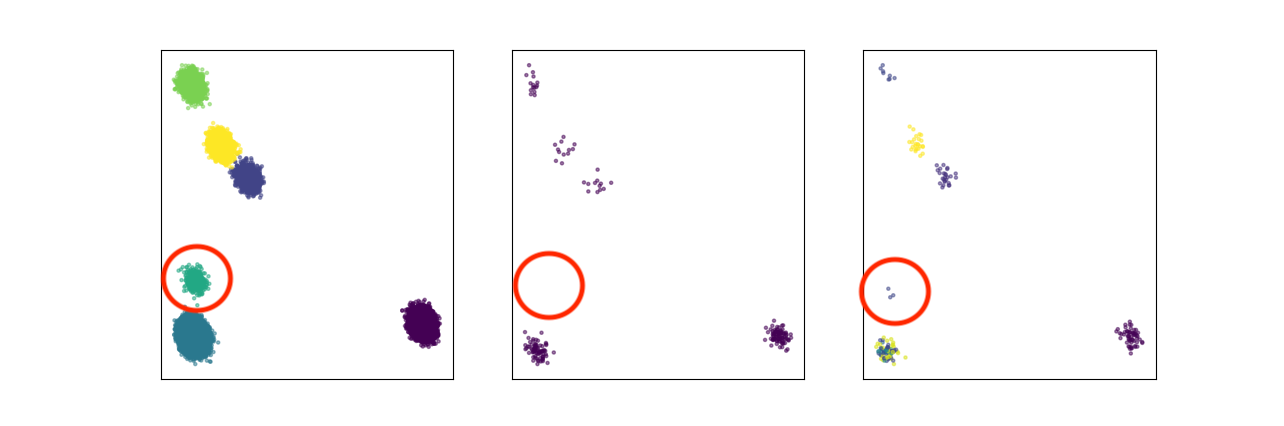
\includegraphics[width=.95\linewidth]{images/lightweight_breaks.png}
\caption{
The results of lightweight and fast-coreset constructions on a dataset of $n=100K$ points with clusters of varying size. Coresets have 200 points.
\emph{Left}: Original multivariate-Gaussian dataset. \emph{Middle}: Lightweight coresets fail to capture the cluster of $\sim$400 points.
\emph{Right}: The Fast-coreset construction runs in linear time but identifies all of the clusters.
}
\end{figure*}


While uniform sampling is expected to be brittle, it may be less obvious what causes light- and welterweight coresets to break. The explanation is simple for
lightweight coresets: they sample according to the $1$-means solution and are therefore biased towards points that are far from the mean. Thus, as a simple
counterexample, lightweight coresets are likely to miss a small cluster that is close to the center-of-mass of the dataset. This can be seen in
Figure~\ref{fig:lightweight_breaks}, where we show an example where the lightweight coreset construction fails on the Gaussian mixture dataset. Since the small
circled cluster is close to the center-of-mass of the dataset, it is missed when sampling according to distance from the mean.

It may be less immediately clear why welterweight coresets are brittle for $j < k$. To understand this, let $\calC_j$ be the approximation obtained during
welterweight coresets and observe that the sum of importance values of the points belonging to center $c_i \in \calC_j$ is \[ \sum_{p \in c_i} \left[
\dfrac{\cost(p, c_i)}{\cost(c_i, \calC_j)} + \dfrac{1}{|c_i|} \right] = \dfrac{\sum_{p \in c_i} \cost(p, c_i)}{\cost(c_i, \calC_j)} + 1 = 2.\] Thus, our
probability mass is distributed across the clusters that have been found in the approximate solution. Naturally, if $j < k$ and we missed a cluster from $\opt$,
there is some set of points that have not received an appropriate probability mass and may therefore be missed.

\begin{table}[htbp]
    \centering
    \small
    \begin{tabular}{lcccc}
        Algorithm & $\gamma = 0$ & $\gamma = 1$ & $\gamma = 3$ & $\gamma = 5$\\
        \hline
        \vspace*{-0.15cm}\\
        LW Coreset & 1.03 & 1.03 & 1.36 & 2.17\\
        $j=2$ & 1.04 & 1.04 & 1.04 & 1.92\\
        $j=\log k$ & 1.04 & 1.04 & 1.04 & 1.95\\
        $j=\sqrt{k}$ & 1.05 & 1.06 & 1.04 & 1.18\\
        Fast Coreset & 1.03 & 1.03 & 1.04 & 1.12\\
        \vspace*{-0.15cm}\\
    \end{tabular}
    \caption{The effect of $\gamma$ in the Gaussian mixture dataset on the coreset distortion. We report the means over 5 random dataset generations.
    Each generation had 50\,000 points in 50 dimensions, with 50 Gaussian clusters and coresets of size 4\,000. We set $k=100$.}
    \label{tbl:class-imbalance}
\end{table}



We evaluate the full extent of this relationship in Table~\ref{tbl:class-imbalance}, where we show the interplay between the welterweight coreset's $j$
parameter (number of centers in the approximate solution) and the Gaussian mixture dataset's $\gamma$ parameter (higher $\gamma$ leads to higher class
imbalance). We can consider this as answering the question ``How good must our approximate solution be before sensitivity sampling can handle class imbalance?''
To this end, all the methods have low distortion for small values of $\gamma$ but, as $\gamma$ grows, only Fast-Coresets (and, to a lesser extent,
welterweight coresets for larger values of $j$) are guaranteed to have low distortion.

\begin{figure}
    \centering
    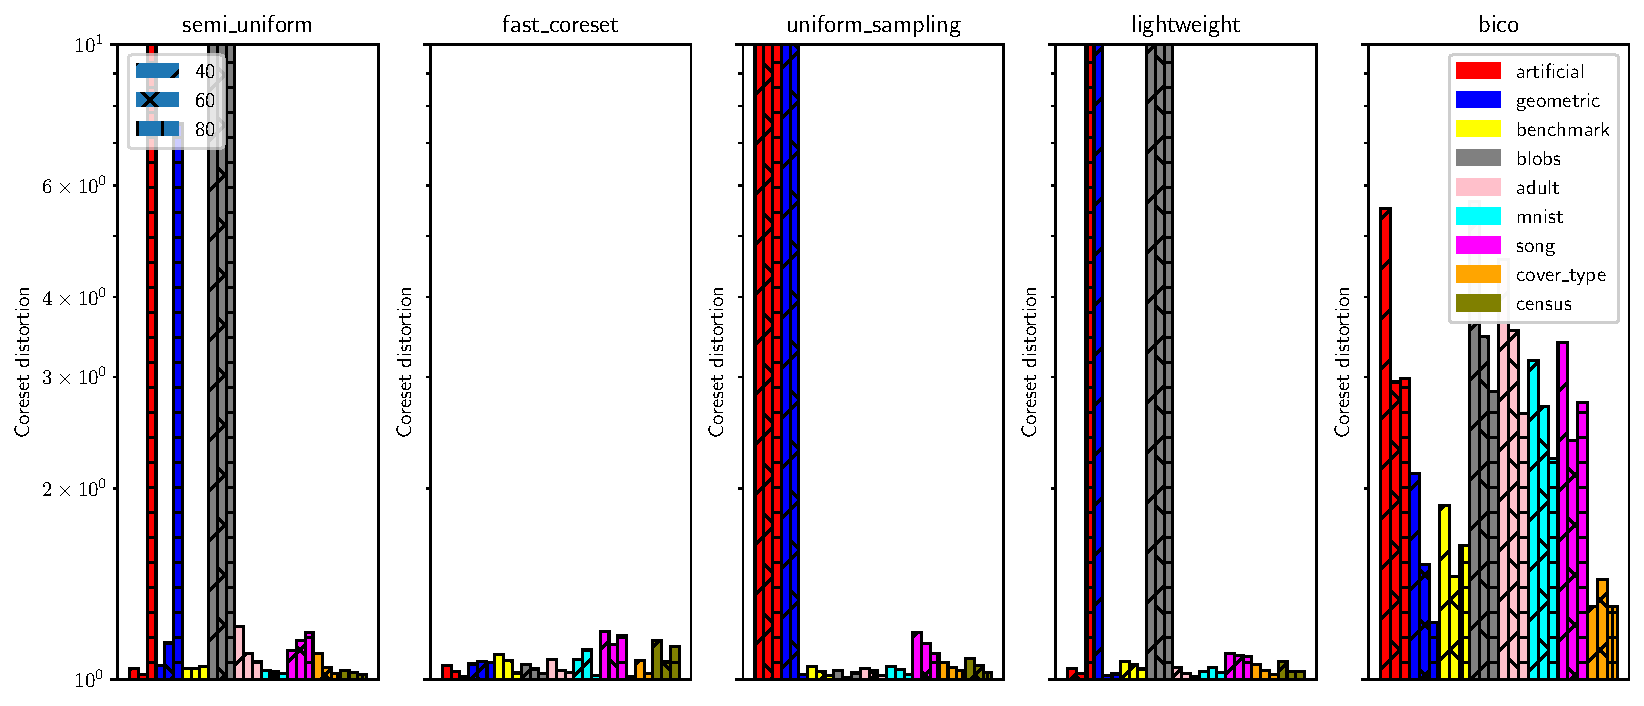
\includegraphics[width=\linewidth]{images/1/coreset_distortion-m_scalar_across_all_algorithms.pdf}
    \vspace*{-0.6cm}
    \caption{Sample coreset distortions under $k$-median for one run on each dataset. Bars within each dataset correspond to $m=40k, 60k, 80k$.}
    \label{subfig:kmedian_distortion}
\end{figure}
For completeness, we verify that these results also hold for the $k$-median task in Figure~\ref{subfig:kmedian_distortion}. There, we see that $k$-median
distortions across datasets are consistent with $k$-means distortions. We show one of five runs to emphasize the random nature of compression quality when using
various sampling schemas.

To round out the dataset analysis, we note that BICO performs consistently poorly on the coreset distortion metric\footnote{We do not include BICO in Figures
\ref{fig:coreset_size_on_quality}, \ref{subfig:kmedian_distortion}, \ref{fig:streaming_runtimes},  as it does not fall into the $\tilde{O}(nd)$ complexity class
and is only designed for $k$-means.}, as can be seen in Tables \ref{tbl:distortion} and \ref{tbl:composition}. We also point out that every sampling method
performs well on the benchmark dataset, which is designed to explicitly punish sensitivity sampling's reliance on the initial solution. Thus, we verify that
there is no worst-case setting which breaks sensitivity sampling as there are for the other sampling methods.  Lastly, we show how these compression schemas
facilitate fast clustering on large datasets in Table~\ref{tbl:lloyds}. There, we see that running Lloyd's algorithm on the samples obtains a consistent cost
value on the full datasets.

\subsection{Streaming Setting}
\label{ssec:streaming}

\begin{figure}
    \centering
    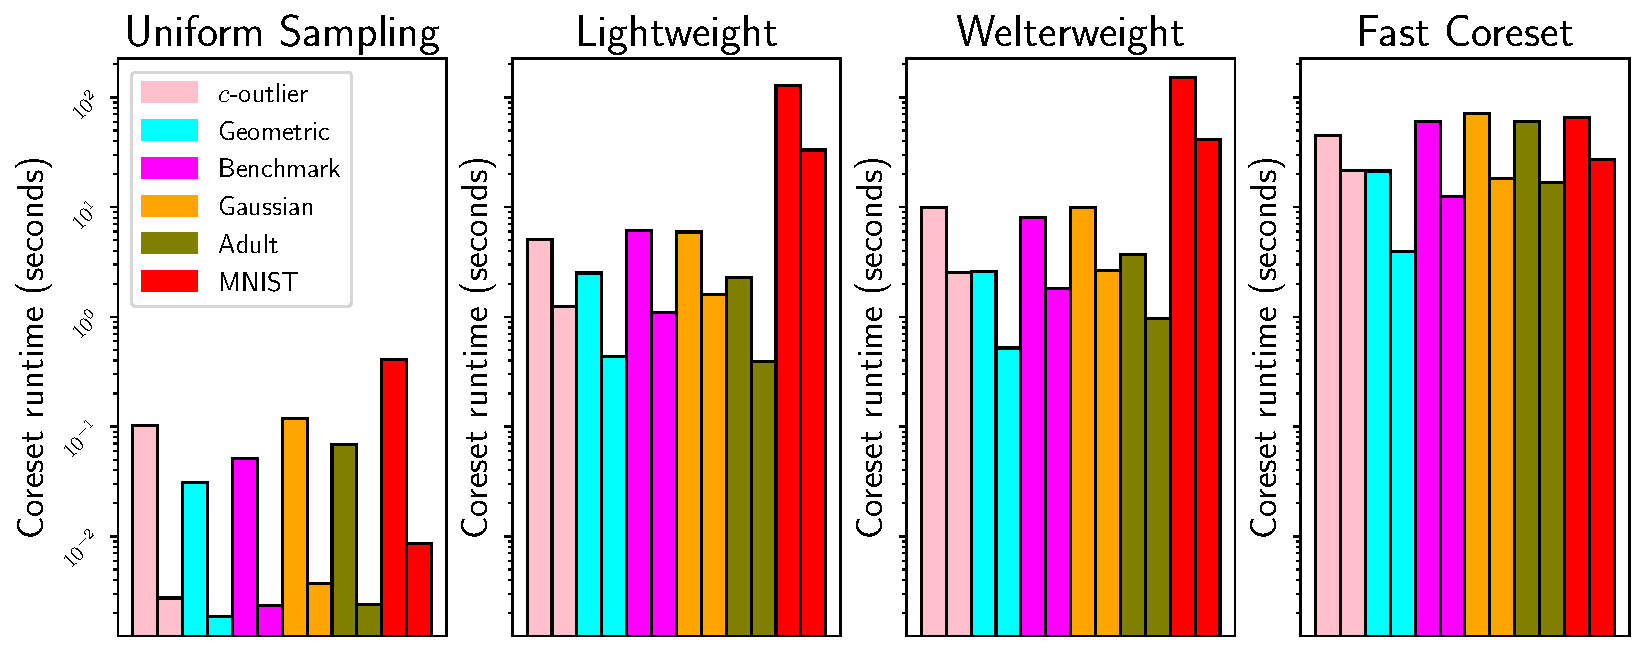
\includegraphics[width=.95\linewidth]{images/2/coreset_runtime-composition.pdf}
    \caption{Mean runtime over three runs in the streaming and non-streaming settings. Bars are [Streaming, Non-Streaming]; y-axis is log-scale.}
    \label{fig:coreset_size_on_sens_quality}
\end{figure}


One of the most common use-cases for big-data algorithms is the streaming setting, where one receives input in batches and must maintain a compression that is
representative of the dataset. Although there is a wealth of sampling and coreset methods in the streaming paradigm, we require consistency across algorithms
and therefore assume a black-box sampling procedure. Since the coreset property is preserved under composition, we utilize the merge-\&-reduce strategy
originally proposed by \cite{BS80} and first applied to maintaining clustering coresets in stream by \cite{HaM04}. The idea is to first partition the input into
$b$ blocks and then perform sampling and composition along them until a single compression is obtained. Specifically, we start by obtaining a coreset on each
block. Then, combining samples using a complete binary tree, we (1) recursively re-sample from the children until there is at least one coreset for each
level\footnote{If there are $b=8$ blocks, then there would be coresets corresponding to blocks $[[1], [2], [3, 4], [5, 6, 7, 8]]$} in the tree and then (2)
concatenate these samples and obtain one final coreset from the composition. Since we are composing coresets from coresets, the errors stack and, in theory, we
should require more samples to obtain a similar accuracy.

Despite this, we see the opposite result for many of our sampling strategies. Surprisingly, Table~\ref{tbl:composition} and Figure~\ref{fig:streaming_runtimes}
show that the accelerated sampling methods all perform \emph{better} under composition on the artificial datasets and do not suffer significant drops in
accuracy, variance or runtime on the real datasets. Although inconsistent with the prevailing intuition, we must therefore conclude that the accelerated
sampling methods are \emph{more} feasible in the streaming setting.  We suspect that this is due to the non-uniformity imposed by the merge-\&-reduce algorithm.
To see this, consider uniform sampling on the $c$-outlier dataset during the final step of the composition, where we are composing the samples corresponding to
each layer of the tree. Assume first that our outlier points happened to fall in the first block. Then we have taken a sample of size $m$ from this block and
immediately use this for the final composition. Thus, in this case the outliers are \emph{more} likely to be in our final sample than in the non-streaming
setting. In the alternate setting where the outliers are less likely, our expected error is already high and missing the outlier `more' cannot worsen our
expected error. 



\section{Conclusion}

In this work, we discussed the theoretical and practical limits of compression algorithms for center-based clustering. We proposed the first nearly-linear time
coreset algorithm for $k$-median and $k$-means. Moreover, the algorithm can be parameterized to achieve an asymptotically optimal coreset size. Subsequently, we
conducted a thorough experimental analysis comparing this algorithm with fast sampling heuristics. In doing so, we find that although the Fast-Coreset algorithm
achieves the best compression guarantees among its competitors, naive uniform sampling is already a sufficient compression for downstream clustering tasks in
well-behaved datasets. Furthermore, we find that intermediate heuristics interpolating between uniform sampling and coresets play an important role in
balancing efficiency and accuracy. 

Although this closes the door on the highly-studied problem of optimally small and fast coresets for $k$-median and $k$-means, open questions of wider scope
still remain. For example, under what conditions does sensitivity sampling guarantee accurate compression in linear-time or of optimal space and can these
generalizations be formalized? Furthermore, sensitivity sampling is incompatible with paradigms such as fair-clustering and it is unclear whether one can
expect that a linear-time method can optimally compress a dataset while adhering to the fairness constraints.




% Acknowledgements should only appear in the accepted version.

\bibliographystyle{plainnat}
\bibliography{references}

\newpage
\appendix
\section{Extensions to \cref{alg:main}} 
\label{app:extensions}
Consider that \cref{alg:main}  only needs to be provided with an assignment to a solution that is a $O(\polylog k)$ approximationone, implying that one could
compute the solution $\calC$ via any algorithm that satisfies this.  This initial solution may as well be an $O\lpar\polylog \lnor P \rnor_0 \rpar$
approximation: using the iterative coreset construction from \cite{BravermanJKW21}, one could then derive a near-optimal coreset size, only suffering
a $O(\log^* n)$ loss in the running time.

As an example, we illustrate a different approach for $k$-median. One could first embed the input into a hierarchically separated tree (HST) with expected
distortion $O(\log \lnor P \rnor_0)$ \cite{FakcharoenpholRT03}. On such tree metrics, solving $k$-median can be done in linear time using dedicated algorithms
(see e.g. \cite{Cohen-AddadLNSS21}). Using the solution from the HST metric, one can compute a coreset, and iterate using the previous argument.  This embedding
into HST is very similar to what is done by the \fkmeans algorithm, but can be actually performed in \emph{any} metric space, not only Euclidean.  For instance,
in a metric described by a graph with $m$ edges, the running time of this construction would be near linear-time $\tilde O(m)$.

\section{Overview of Quadtree Construction}
\label{app:quadtree}

The first step is to obtain a box enclosing all input points, centered at zero, with all side lengths equal to
$\boxsize$. This can be done as follows: select an arbitrary input point, and translate the dataset so that this point is at the origin. Then, using
$O(nd)$ time, set $\boxsize$ to be the maximum distance from any point to the origin. Having obtained this box, add a random shift $s \leq \boxsize$ is to all the points'
coordinates so that the input is now in the box $[-2\boxsize, 2\boxsize]^d$. This transformation does not change any distances and therefore preserves the
$k$-median cost.  The $i$-th level of the tree (for $i \in \lbra 0, ..., \log \Delta \rbra$) is constructed by centering a grid of side length $2^{-i} \cdot
2\boxsize$ at $0$, making each grid-cell a node in the tree.  The parent of a cell $c$ is simply the cell at level $i-1$ that contains $c$, and the distance
between $c$ and its parent is set to $2^{-i} \cdot 2\boxsize \cdot \sqrt{d}$ (the length of the hypercube's diagonal). This embedding takes $O(nd \log \Delta)$
time to construct, where $\log \Delta$ is the depth of the tree.

\section{Proof of \cref{sec:theory}}\label{app:theory}

We formalize the proof that the \cref{alg:main} produces an $\eps$-coreset in time $\tilde O(nd \log \Delta)$
\begin{proof}
%We show that \cref{alg:main} has the desired guarantees.
First, performing the Johnson-Lindenstrauss embedding takes time $\tilde O(nd)$.

On the projected dataset, the algorithm \fkmeans runs in time $\tilde O\lpar n \log \Delta\rpar$, and the solution it has an approximation-ratio $O\lpar \tilde{d}^z \log k\rpar = O\lpar\log^{z+1} k\rpar$ for $\tilde P$. 
The guarantee offered by the embedding ensure that the clustering $\lbra \calC_1,...,\calC_k\rbra$ still has approximation ratio for $P$ \cite{makarychev2019performance}. 

For $k$-means, computing the $1$-mean solution for each $\calC_i$ takes time $O(nd)$ (the $1$-mean is simply the mean). 
For $k$-median, computing the $1$-median solution can be done as well in time $O(nd)$ \cite{CohenLMPS16}. 
We note that both may be approximated to a factor $2$ in constant time, by sampling uniformly at randm few points from each cluster \cite{neurips21}.

Provided the $c_i$ and the partition $\calC_i$, computing $|\calC_i|$ and $\cost(\calC_i, c_i)$ for all $i$ also takes time $O(nd)$.

Since the solution consisting of assigning each $p \in \calC_i$ to $c_i$ is a $O\lpar \log^{z+1} k\rpar$-approximation, the values $s(p)$ defined in \cref{alg:main} can be used to perform the coreset construction algorithm, and we conclude from \cref{fact:logApprox}.
\end{proof}


\subsection{Reduction to $k$-median.}
\label{app:redKM}

\begin{lemma}
Let $\calS$ be a $c$-approximation for $k$-median on $P$. Then, $\calS$ is a $nc^2$-approximation for $k$-means on $P$.
\end{lemma}
\begin{proof}
Let $\cost_1$ (resp. $\cost_2$) be the $k$-median (resp. $k$-means) cost, $\opt_1$ (resp. $\opt_2$) be the optimal $k$-median (resp. $k$-means) solution. We have the following inequalities:
\begin{align*}
\cost_2(\calS) &= \sum_{p\in P} \dist(p, \calS)^2 \leq \lpar \sum_{p\in P} \dist(p, \calS)\rpar^2\\
&\leq c^2 \cdot \lpar  \sum_{p\in P} \dist(p, \opt_1)\rpar^2\\
&\leq c^2 \cdot \lpar  \sum_{p\in P} \dist(p, \opt_2)\rpar^2\\
&\leq c^2 \cdot n \cdot  \sum_{p\in P} \dist(p, \opt_2)^2,
\end{align*}
where the last inequality stems from Cauchy-Schwarz. Therefore, $\calS$ is a $nc^2$ - approximation to $k$-means. 
\end{proof}


\subsection{Estimation of the Optimal Cost in a Tree}
\label{app:apx-tree-proof}

\begin{proof}[proof of \cref{lem:apxTree}]
If the input is spread in $k+1$ distinct cell at level $i$, then in any solution there is at least one of those cells with no center. In the tree metric, points lying in this cell have therefore connexion cost at least $\sqrt{d}2^{-i+1} \cdot \boxsize$, and thus the left-hand-side of the inequality holds.

On the other hand, if the input is contained into $k$ cells at level $i-1$, then placing arbitrarily a center in each cell yields a solution with cost at most $n \cdot \sqrt{d}2^{-i+4} \cdot \boxsize$: indeed, the distance from any point to its closest center is at most $2 \cdot \sum_{j \geq i-1} \sqrt{d}2^{-j} \cdot 2\boxsize \leq 4 \sqrt{d}2^{-i+2} \cdot \boxsize$ (summing the edge length from the point to the cell at level $i$, and then going down to the center). This concludes.
\end{proof}

\begin{figure*}
\label{fig:lightweight_breaks}
\centering
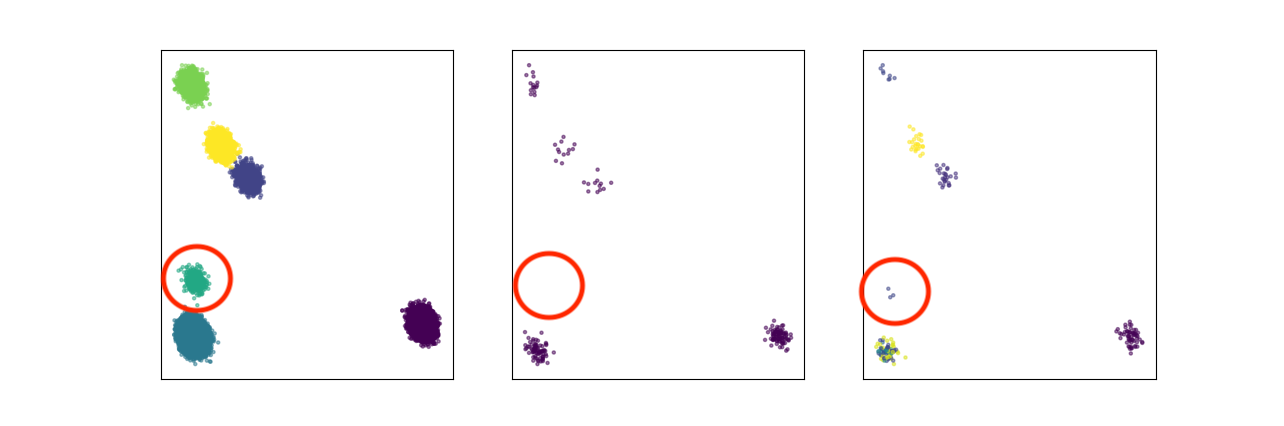
\includegraphics[width=.95\linewidth]{images/lightweight_breaks.png}
\caption{
The results of lightweight and fast-coreset constructions on a dataset of $n=100K$ points with clusters of varying size. Coresets have 200 points.
\emph{Left}: Original multivariate-Gaussian dataset. \emph{Middle}: Lightweight coresets fail to capture the cluster of $\sim$400 points.
\emph{Right}: The Fast-coreset construction runs in linear time but identifies all of the clusters.
}
\end{figure*}

\begin{figure}
    \centering
    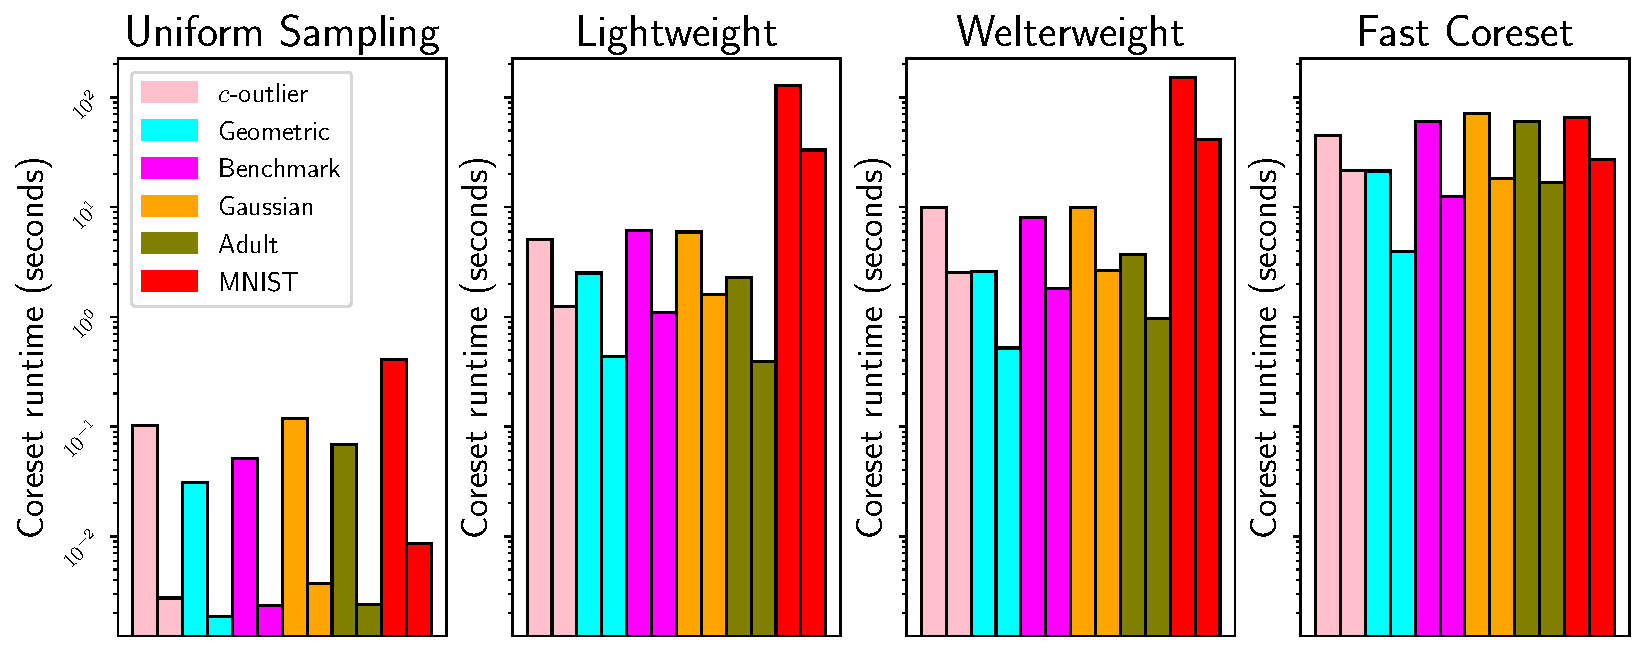
\includegraphics[width=.95\linewidth]{images/2/coreset_runtime-composition.pdf}
    \caption{Mean runtime over three runs in the streaming and non-streaming settings. Bars are [Streaming, Non-Streaming]; y-axis is log-scale.}
    \label{fig:coreset_size_on_sens_quality}
\end{figure}


\section{Data Parameters}
\label{app:data_params}
In all real and artificial datasets, we add random uniform noise $\eta$ with $0 \leq \eta_i \leq 0.001$ in each dimension in order to make all points unique.
Unless specifically varying these parameters, we default all algorithms in~\ref{ssec:algorithms} to $k=100$ for the Adult, MNIST, and artificial datasets and
$k=500$ for the Song, Cover Type, and Census datasets. Our default coreset size is then $m = 40k$. We refer to the coreset size scalar as the \emph{$m$-scalar}.
We only run the dimension-reduction step on the MNIST dataset, as the remaining datasets already have sufficiently low dimensionality.

\begin{table}[htbp]
    \centering
    \begin{tabular}{lrr}
        Dataset & Points & Dim \\
        \hline
        \emph{Adult} & 48\,842 & 14 \\
        \emph{MNIST} & 60\,000 & 784 \\
        \emph{Song} & 515\,345 & 90 \\
        \emph{Cover Type} & 581\,012 & 54 \\
        \emph{Census} & 2\,458\,285 & 68 \\
        \hline
        \vspace*{0.1cm}
    \end{tabular}
    \caption{Description of real world datasets}
    \label{tbl:datasets}
\end{table}


\end{document}
